\chapter{Desenvolvimento}
\label{metodo}

\section{Biblioteca de manipulação de grafos}
Como primeira etapa foi desenvolvida uma biblioteca de manipulação de grafos que será utilizada futuramente nas próximas
etapas.

A biblioteca de manipulação é composta por um conjunto de funções e métodos que manipulam tanto um grafo representado
em matriz, quanto um grafo representado por lista de adjacência.

Para um bom design de solução, que fosse reutilizável e compreensível, foi utilizada a linguagem Java como principal
ferramenta. A arquitetura desenvolvida para a biblioteca, nos dá a liberdade para escolher qual estrutura de dados
manipular e utilizar de módulos de geração, leitura e salvamento de grafos de maneira separada.

A Biblioteca como um todo é composta por duas classes principais que guardam as estruturas de dados de Grafos em matriz
e em lista de adjacência. A primeira classe é chamada de GraphMatrix, responsável por manipular e armazenar um grafo
não-direcionado em uma matriz de N linhas por N colunas tal que N é o número de vértices do grafo. A segunda classe
se chama apenas Graph e ela herda todas as características de GraphMatrix. Graph, é responsável por manipular e
armazenar tanto grafo em matriz, quanto o grafo em lista de adjacência.

Além das classes principais, existem outros dois módulos que auxiliam nos testes e desenvolvimento. Sendo o primeiro
deles chamado de GraphIO, utilizado na leitura e salvamento de grafos em arquivos no formato Pajek NET, e o segundo
módulo, chamado de GraphGenerator, responsável por gerar grafos com base na quantidade de vértices, número mínimo de
grau por vértice e número máximo de grau por vértice.

Para garantir que todos os algoritmos estão funcionando corretamente e retornando resultados esperados, foram
desenvolvidas baterias de teste para cada uma das funções do sistema. Assim, é possível ter certeza e confiar que
tanto o processamento que ocorre nas matrizes, quanto os que ocorrem nas listas entregam os mesmos resultados de
adição e remoção de arestas, ponderação de vértices e arestas, e para todas as outras funções. Os testes foram
escritos utilizando a biblioteca Junit do próprio Java.

A Organização de todo o sistema pode ser representada pelo seguinte diagrama de classe:

\begin{figure}[H]
	% Alterar espaçamentos antes e depois do caption
	\setlength{\abovecaptionskip}{0pt}
	\setlength{\belowcaptionskip}{0pt}
	% Caption
	\caption[Diagrama de Classe]{Diagrama de Classe}
	\centering
	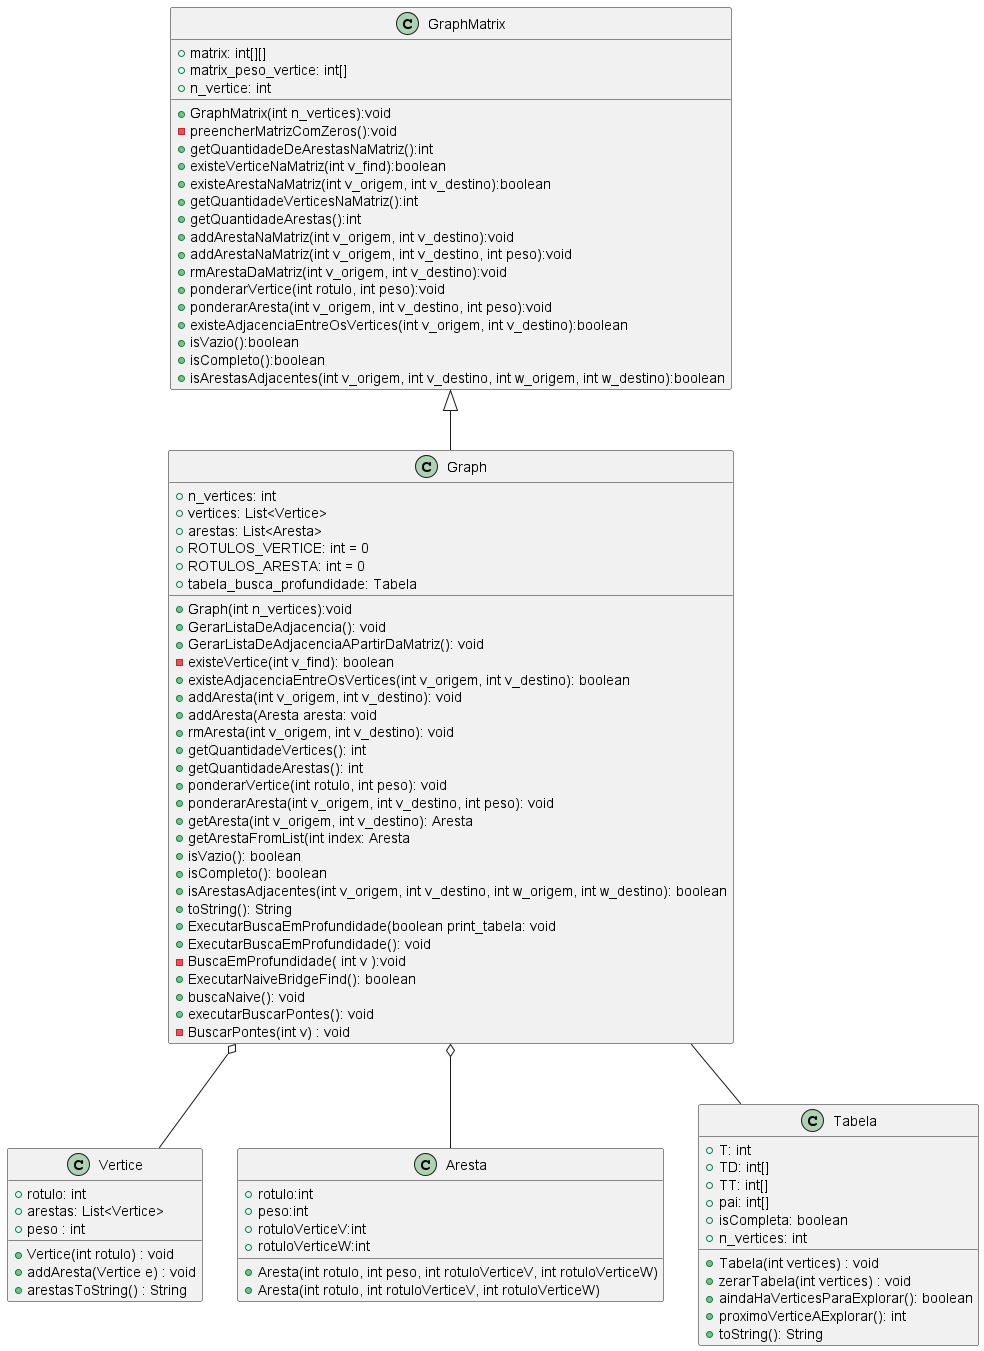
\includegraphics[width=1\textwidth]{DiagramaDeClasse/DiagramaDeClasse.png}
	% Caption centralizada
	\captionsetup{justification=centering}
	%\captionfont{\small{\textbf{\\Fonte: }}}}	
	\label{fig:DiagramaDeClasse}
\end{figure}

\section{Ciclo Euleriano}


Passa uma única vez por cada aresta no grafo, partindo e chegando a um mesmo vértice.

\begin{itemize}
	\item Para haver um ciclo euleriano, todo vértice deve ter grau par, como já discutimos.
\end{itemize}

O algoritmo de Fleury, proposto em 1883, utiliza um grafo reduzido induzido pelas arestas ainda não marcadas

\begin{itemize}
	\item Inicialmente todas as arestas estão não marcadas.
	\item As arestas vão sendo "marcadas", ou removidas do grafo, a medida em que vão sendo inseridas no ciclo
\end{itemize}

Regra da ponte: se uma aresta {v, w} é uma ponte no grafo reduzido, então {v, w} só deve ser escolhida caso não haja outra opção.

\section{Algoritmo de Fleury}

Passo a passo para um grafo não dirigido e não valorado

\begin{enumerate}
	\item Verifique se o grafo apresenta as condições para ter um ciclo euleriano
	\item Caso positivo, escolha um vértice V1 para começar.
	\item Entre os vértices adjacentes a V1, faça
	      \begin{enumerate}
		      \item Se há apenas um vértice como opção, escolha este como V2.
		      \item Se há mais de um vértice possível, escolha um V2 apropriado dentre eles (ou seja, um que “não repita a ponte”).
	      \end{enumerate}
	\item Remova a aresta (V1, V2).
	\item Se ainda houver arestas não percorridas, volte ao passo 3, partindo agora de V2 (V2 é o novo V1).
	\item Caso contrário, imprima o caminho percorrido.
\end{enumerate}

Exemplos do passo a passo do algoritmo funcionando:

\begin{figure}[H]
	\begin{subfigure}{.6\textwidth}
		\centering
		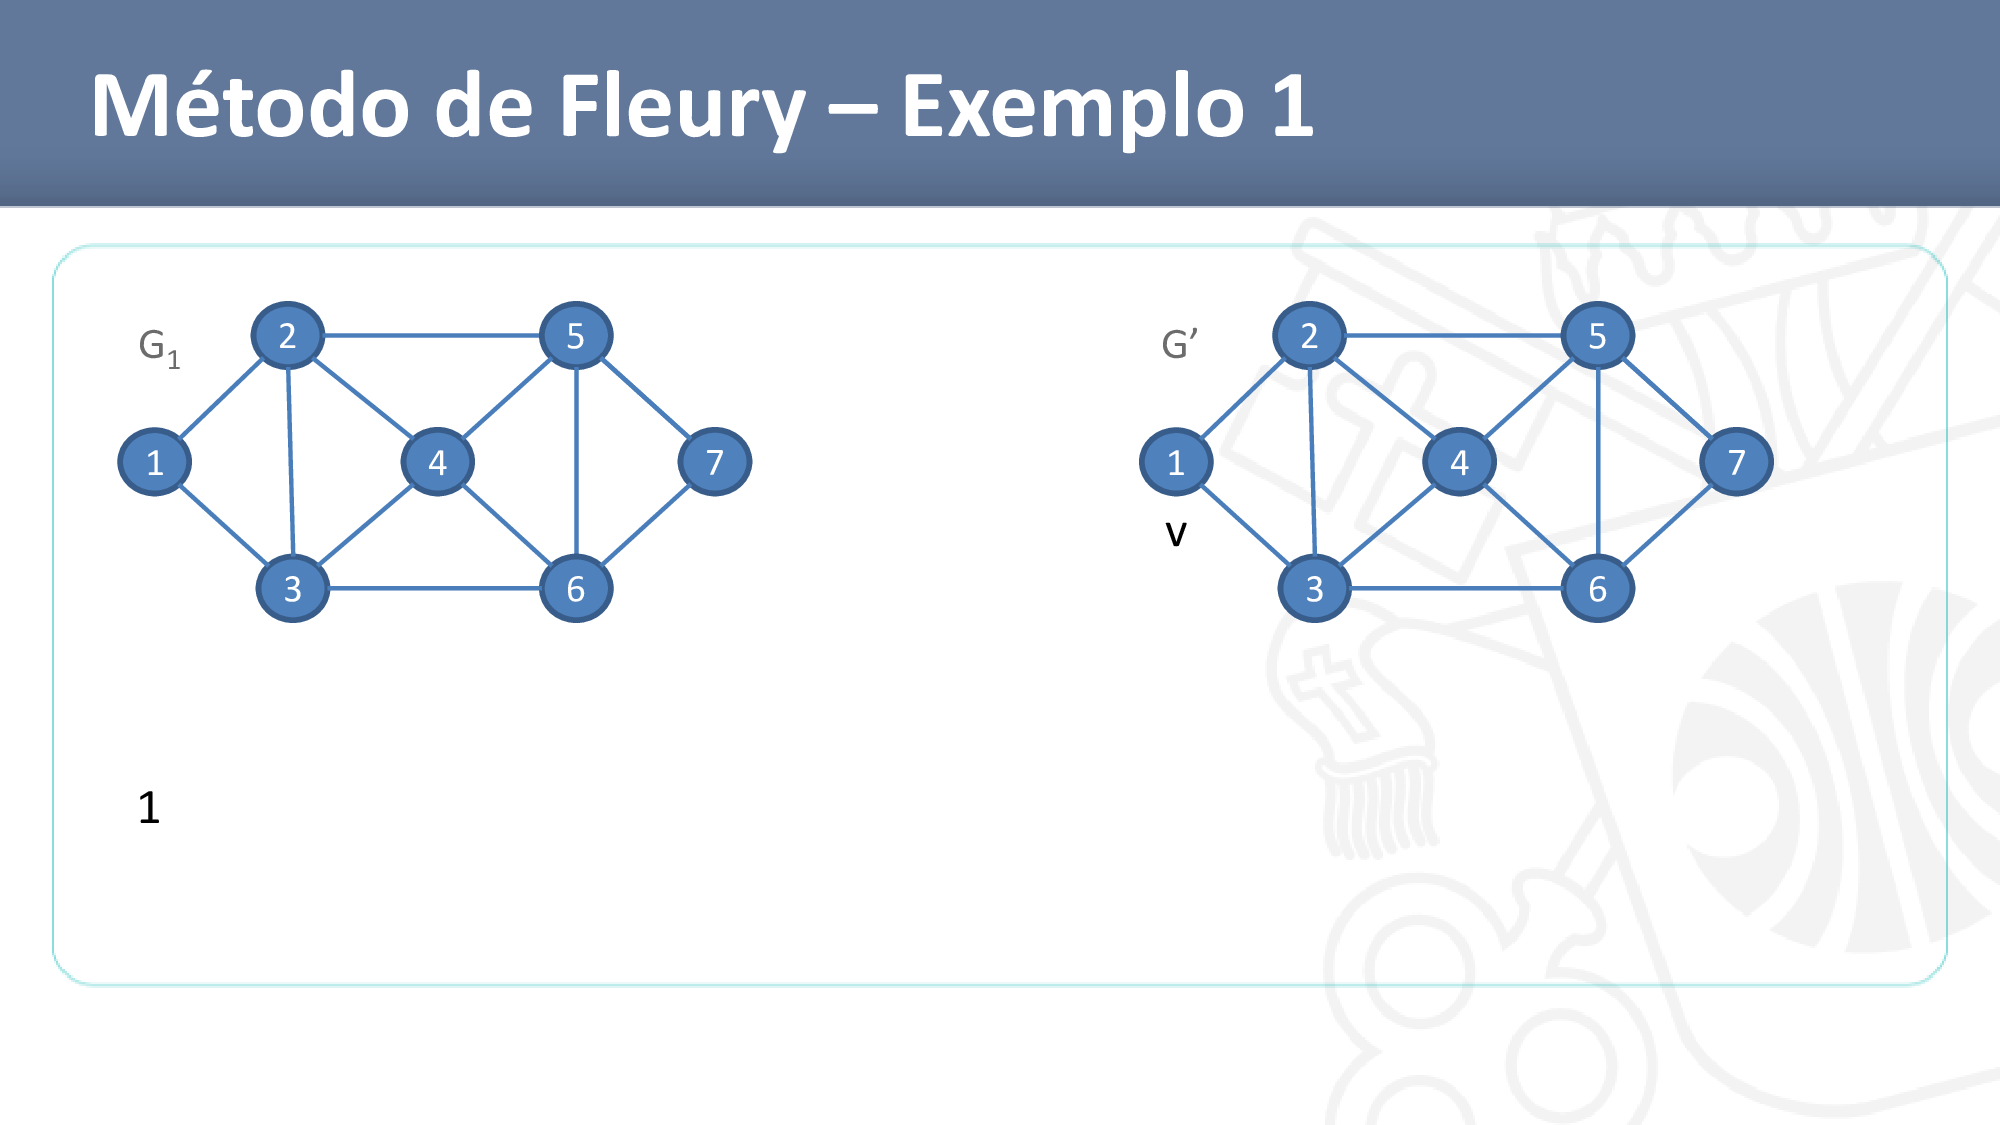
\includegraphics[width=\textwidth]{imagem/graficos/1a1455b7b9174768d1c6a0d41673e79dHTztESkzBtQzsXWu-25.png}
	\end{subfigure}
	\begin{subfigure}{.6\textwidth}
		\centering
		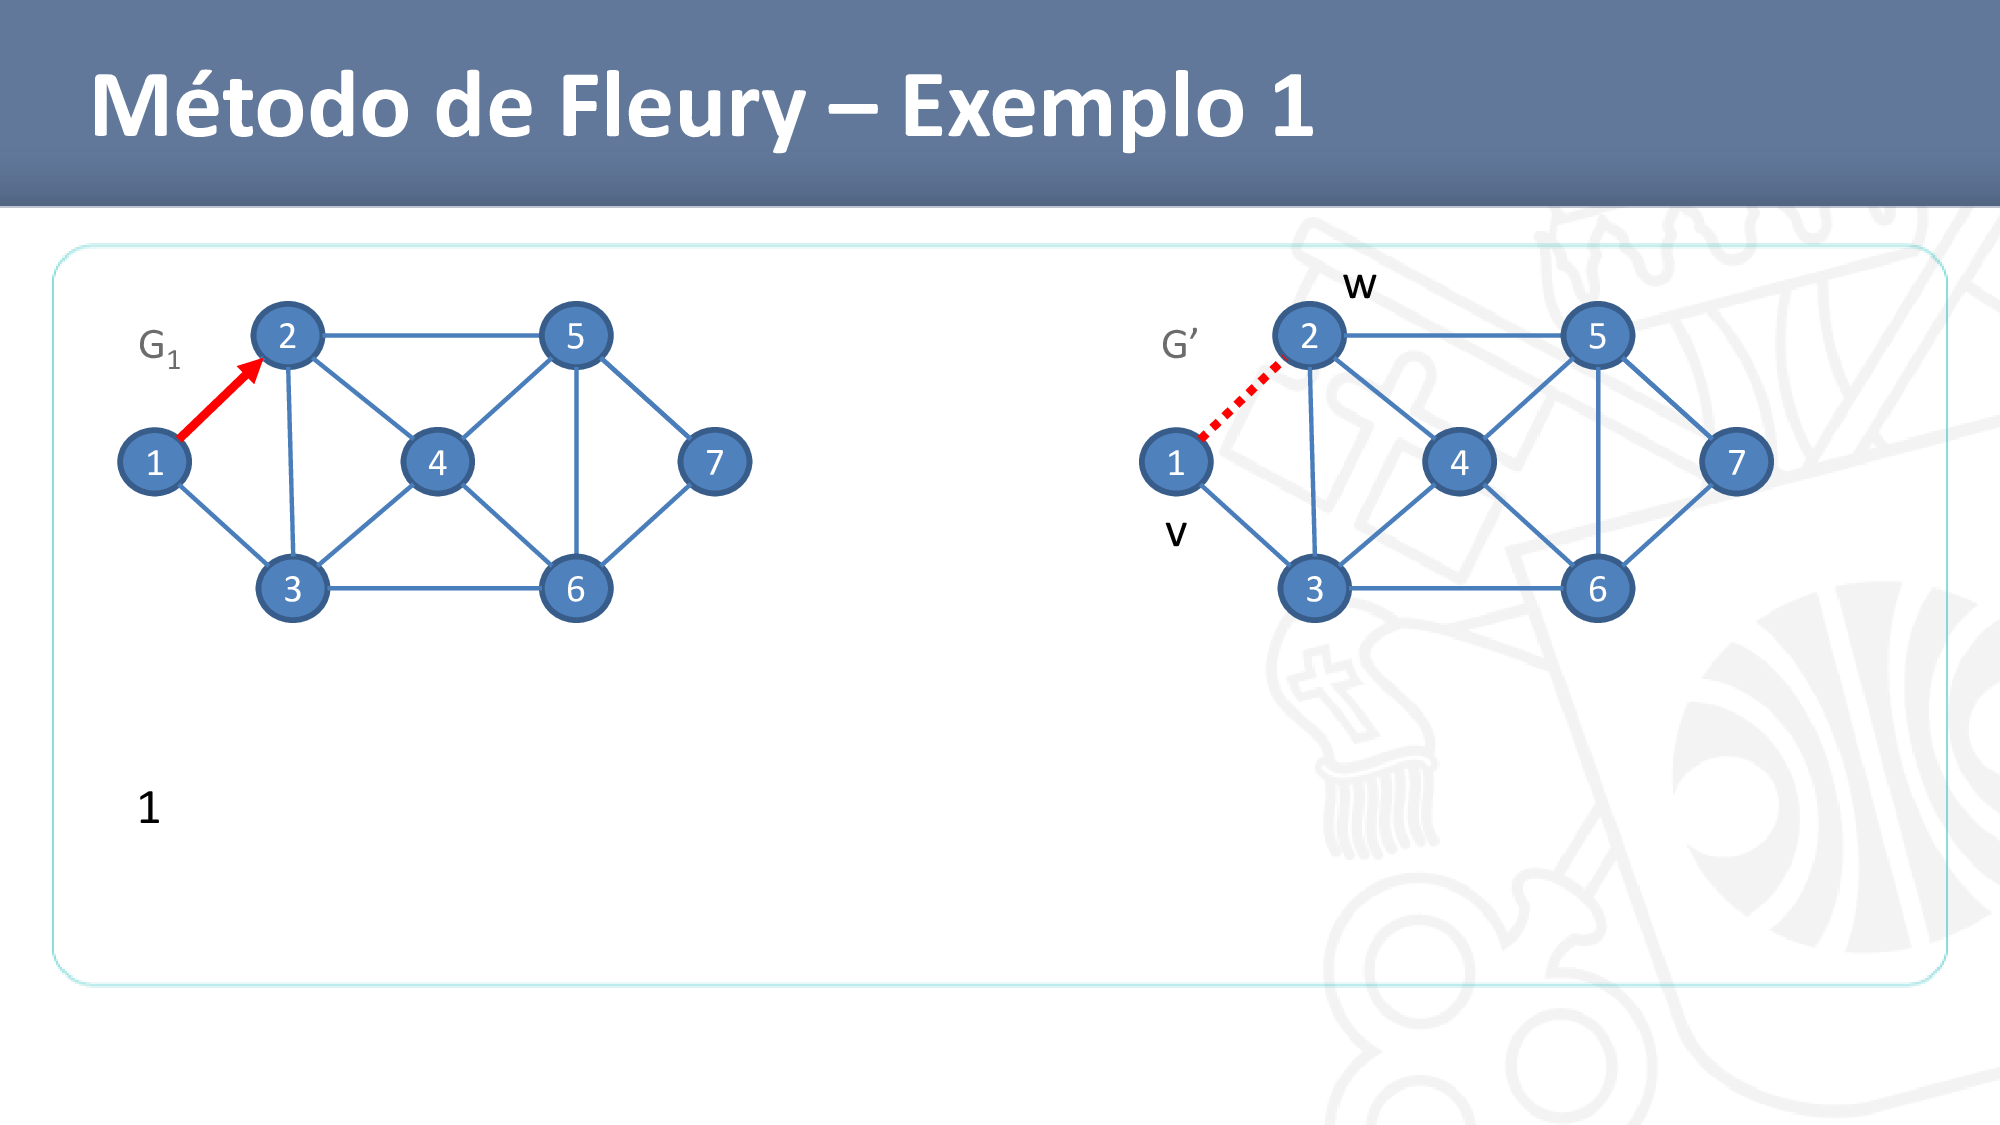
\includegraphics[width=\textwidth]{imagem/graficos/1a1455b7b9174768d1c6a0d41673e79dHTztESkzBtQzsXWu-26.png}
	\end{subfigure}
\end{figure}
\begin{figure}[H]
	\begin{subfigure}{.6\textwidth}
		\centering
		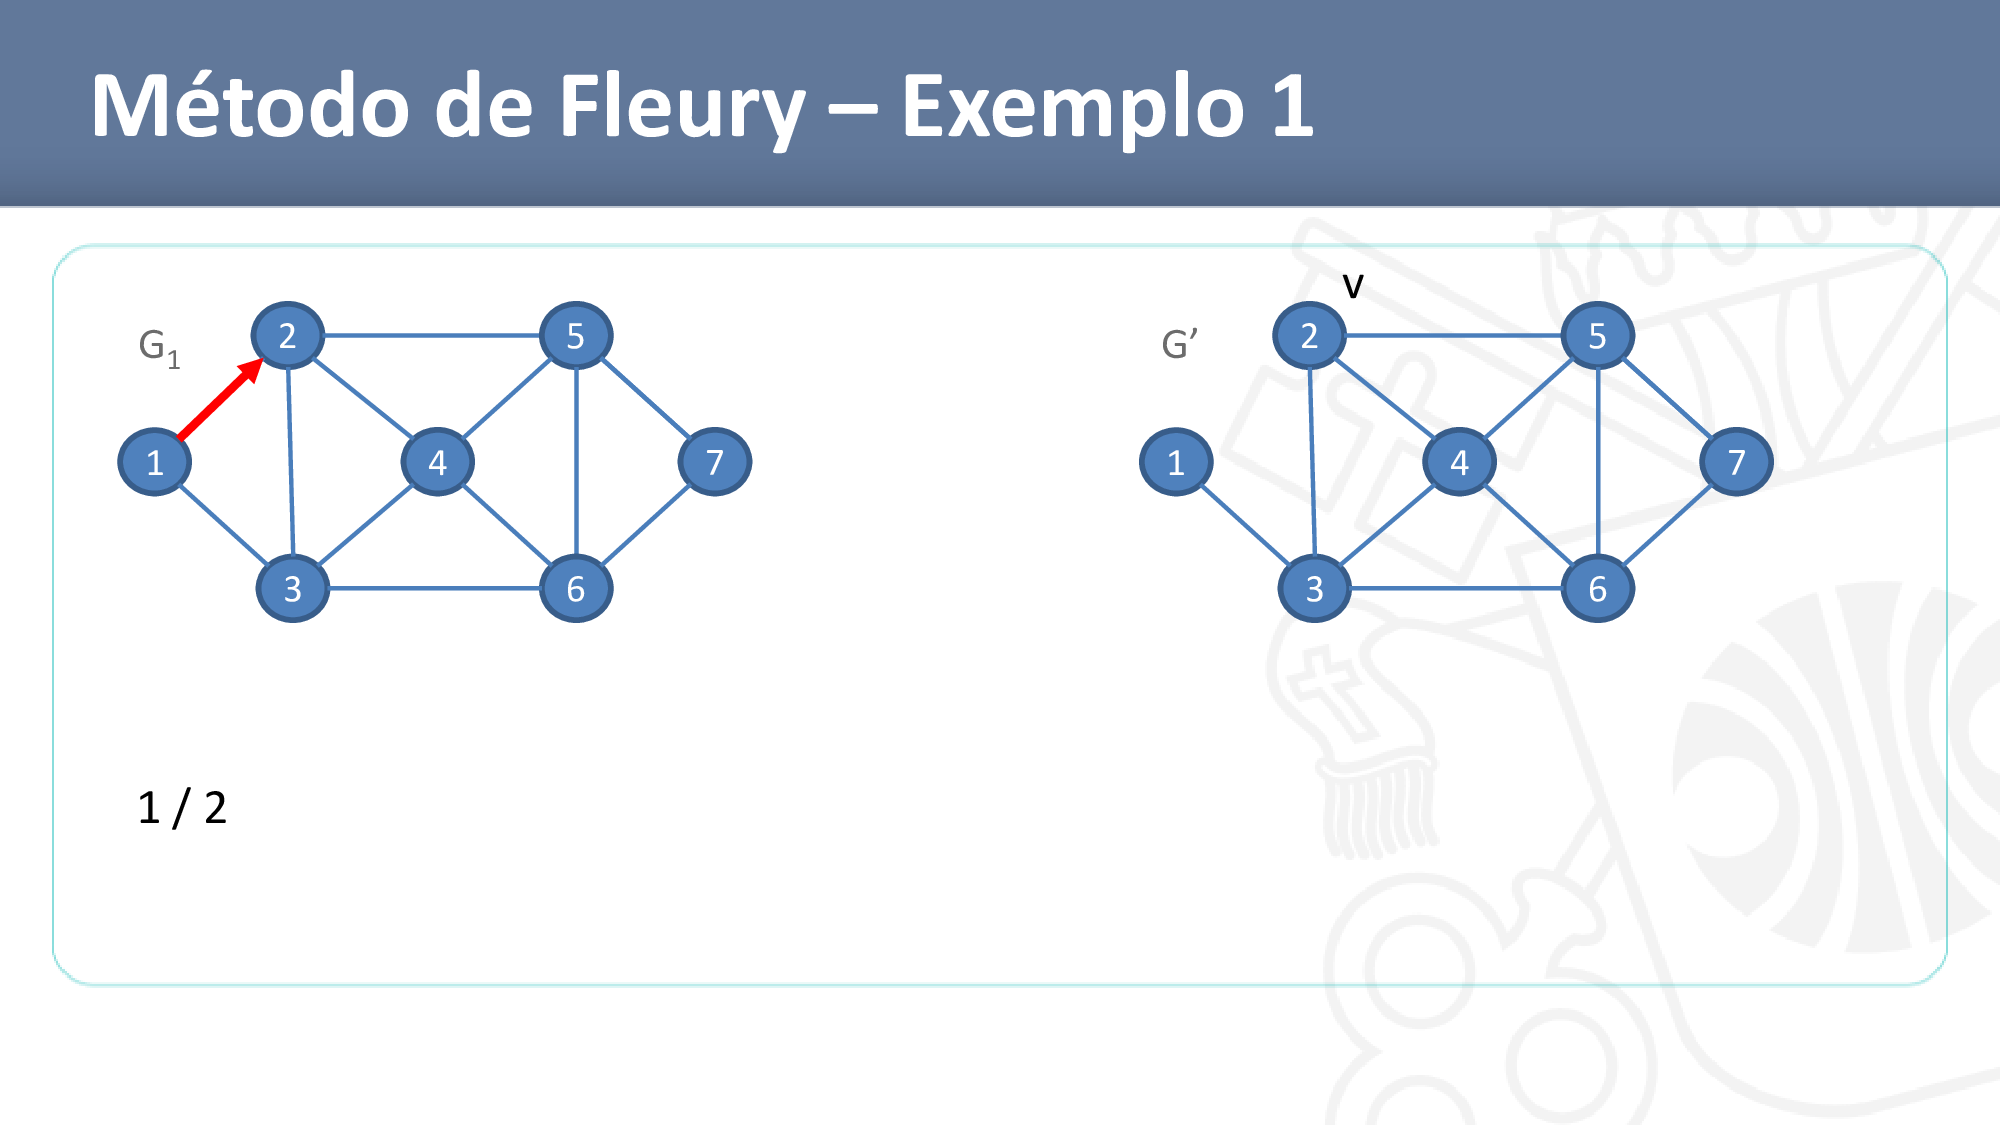
\includegraphics[width=\textwidth]{imagem/graficos/1a1455b7b9174768d1c6a0d41673e79dHTztESkzBtQzsXWu-27.png}
	\end{subfigure}
	\begin{subfigure}{.6\textwidth}
		\centering
		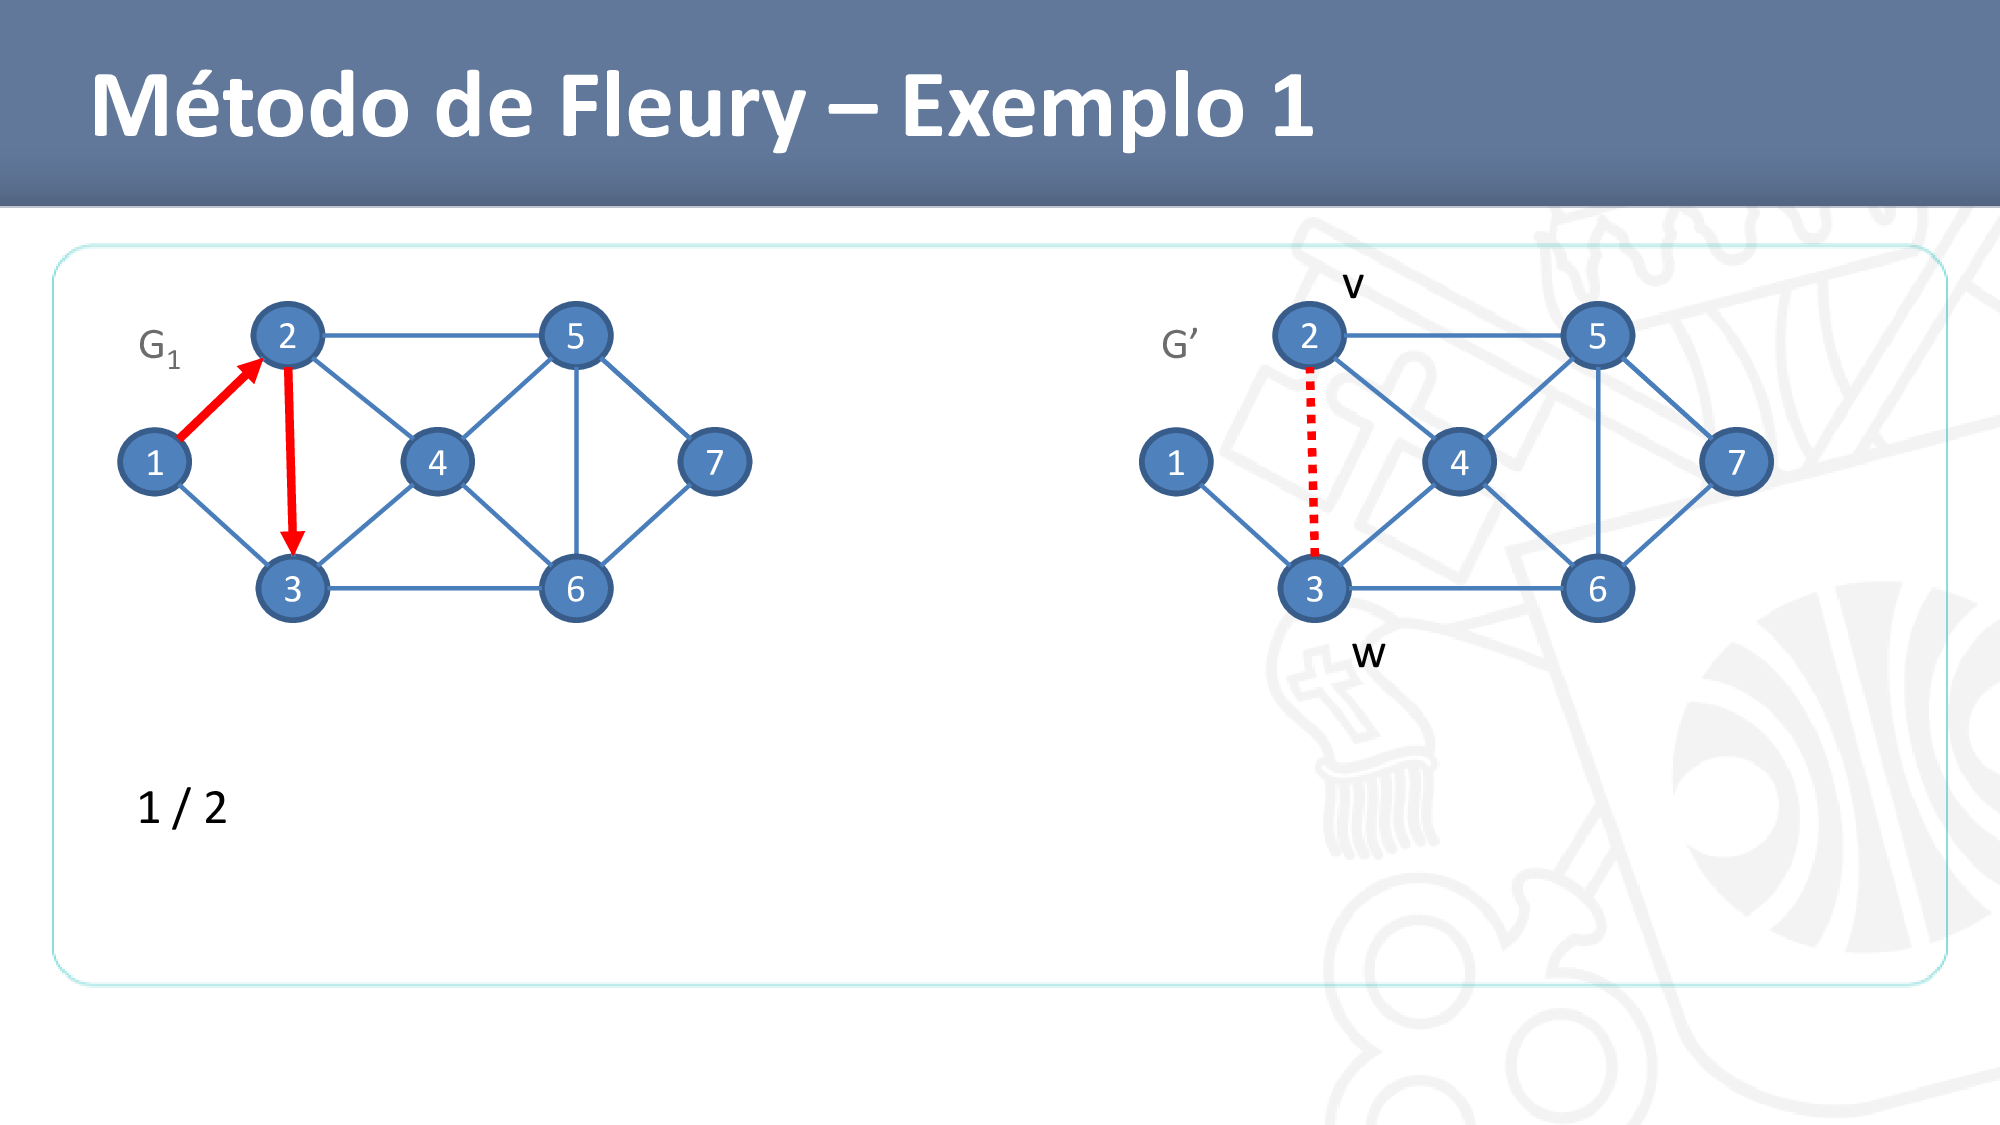
\includegraphics[width=\textwidth]{imagem/graficos/1a1455b7b9174768d1c6a0d41673e79dHTztESkzBtQzsXWu-28.png}
	\end{subfigure}
\end{figure}
\begin{figure}[H]
	\begin{subfigure}{.6\textwidth}
		\centering
		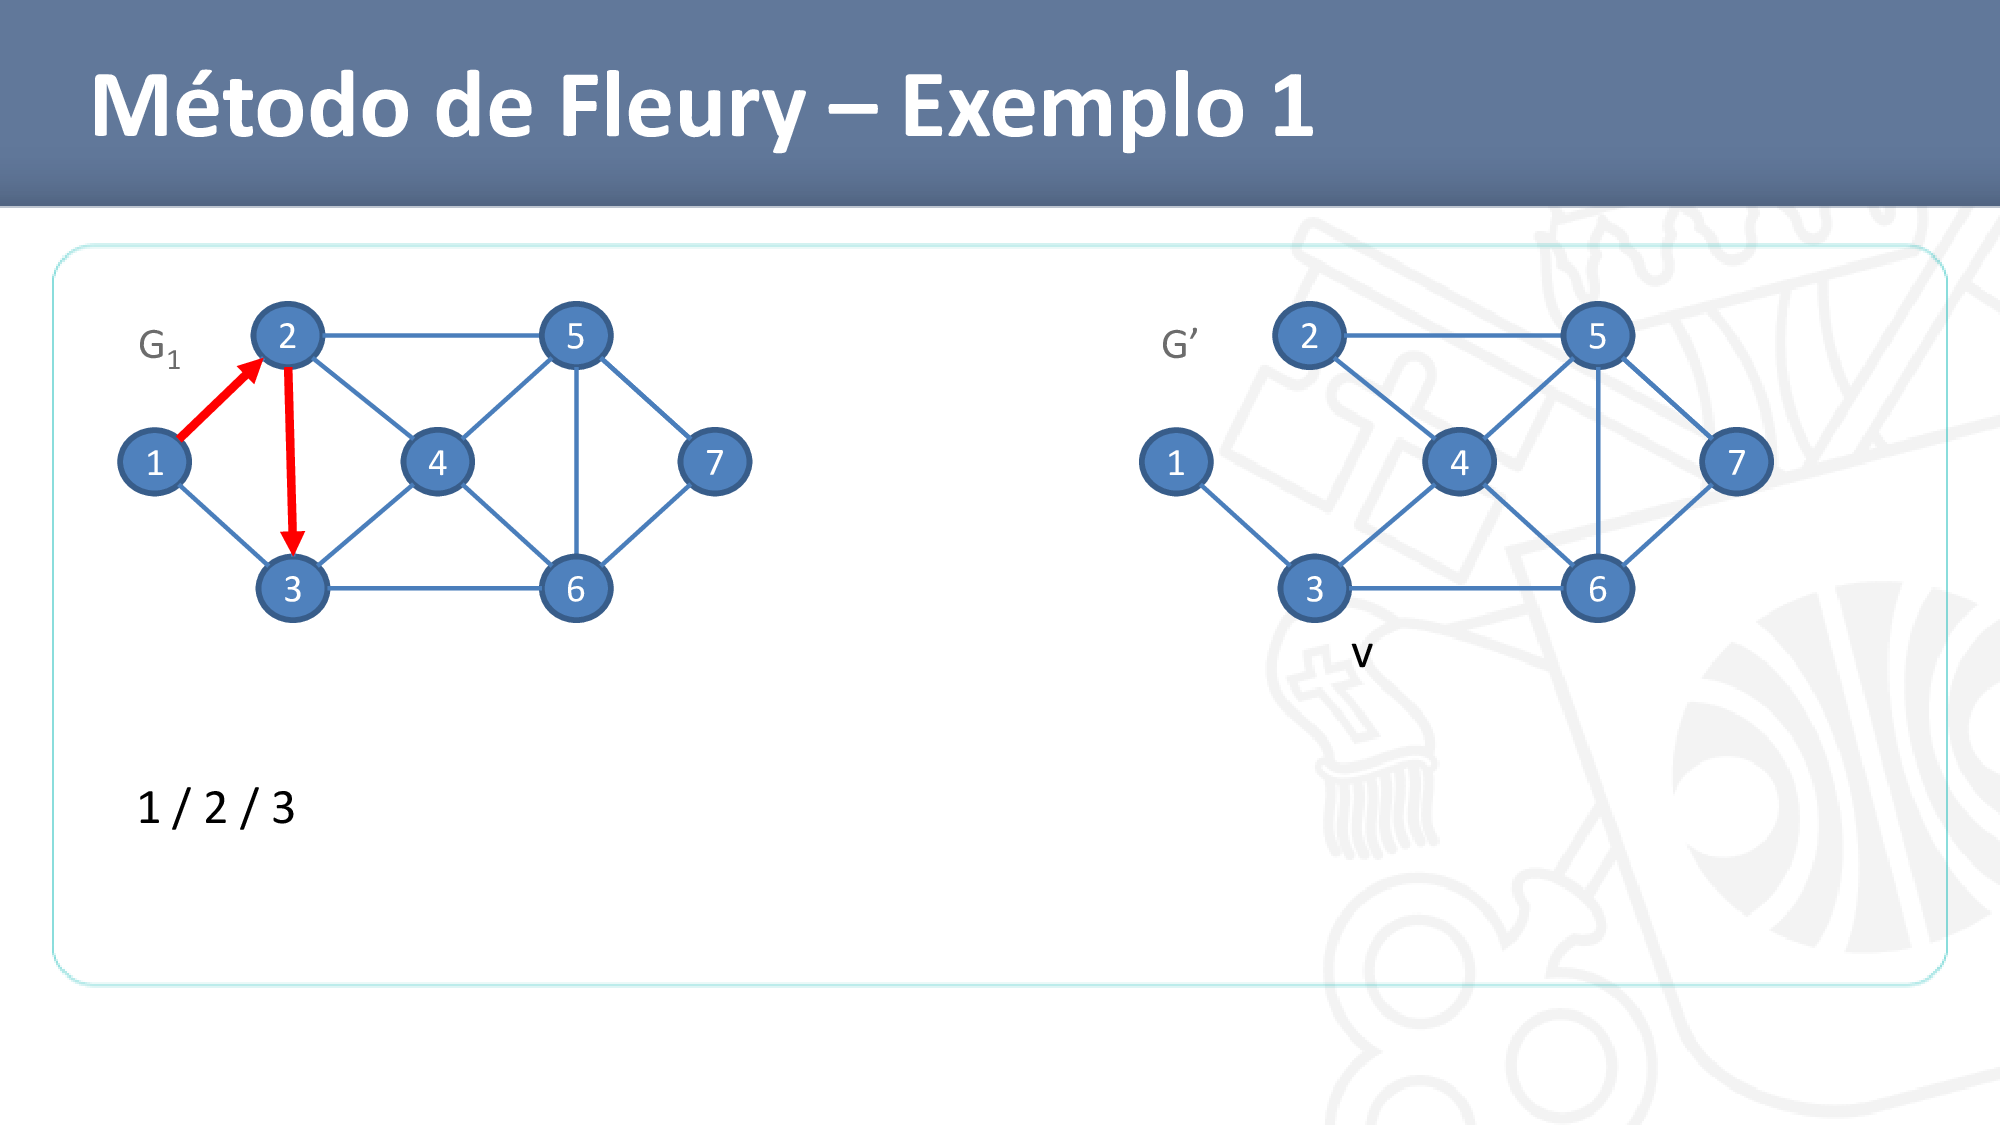
\includegraphics[width=\textwidth]{imagem/graficos/1a1455b7b9174768d1c6a0d41673e79dHTztESkzBtQzsXWu-29.png}
	\end{subfigure}
	\begin{subfigure}{.6\textwidth}
		\centering
		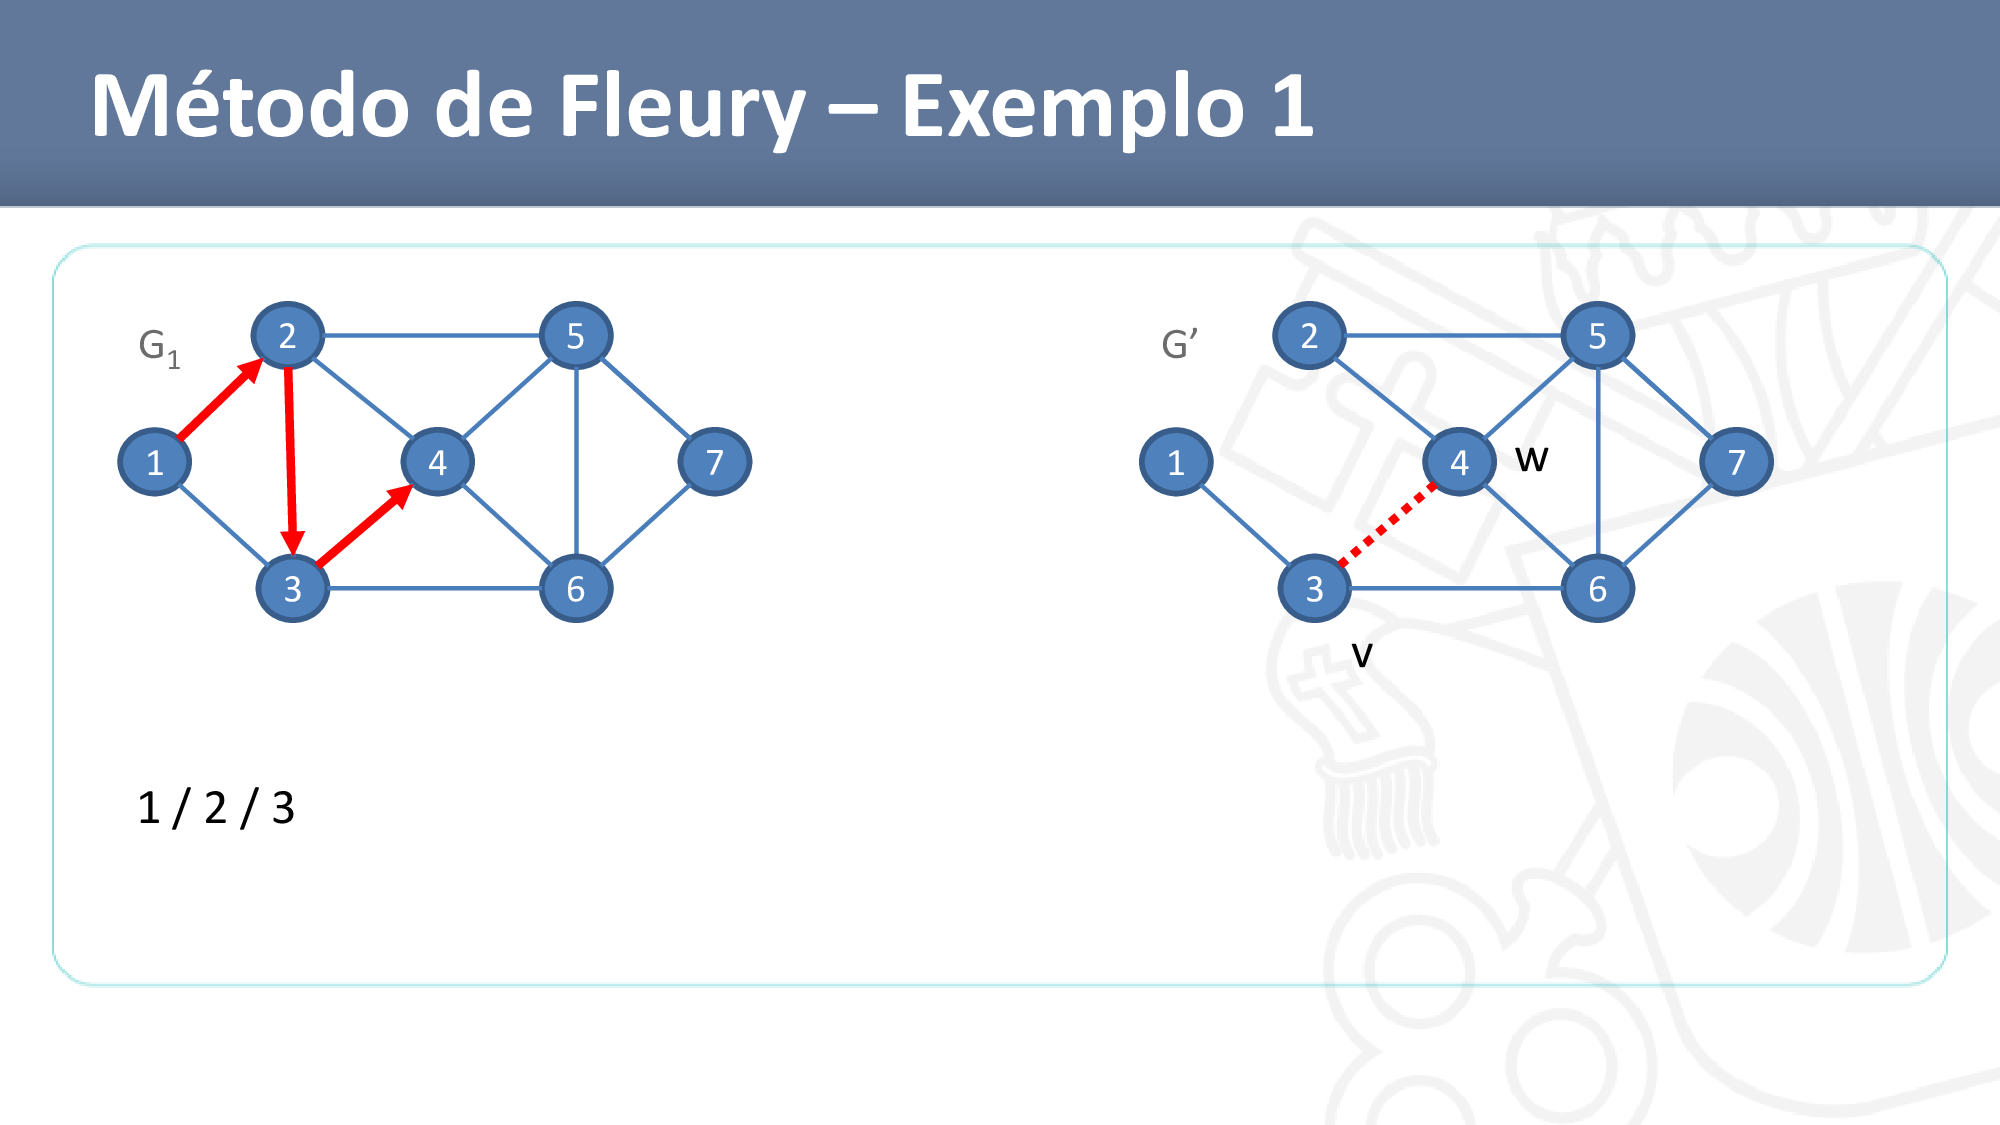
\includegraphics[width=\textwidth]{imagem/graficos/1a1455b7b9174768d1c6a0d41673e79dHTztESkzBtQzsXWu-30.png}
	\end{subfigure}
\end{figure}
\begin{figure}[H]
	\begin{subfigure}{.6\textwidth}
		\centering
		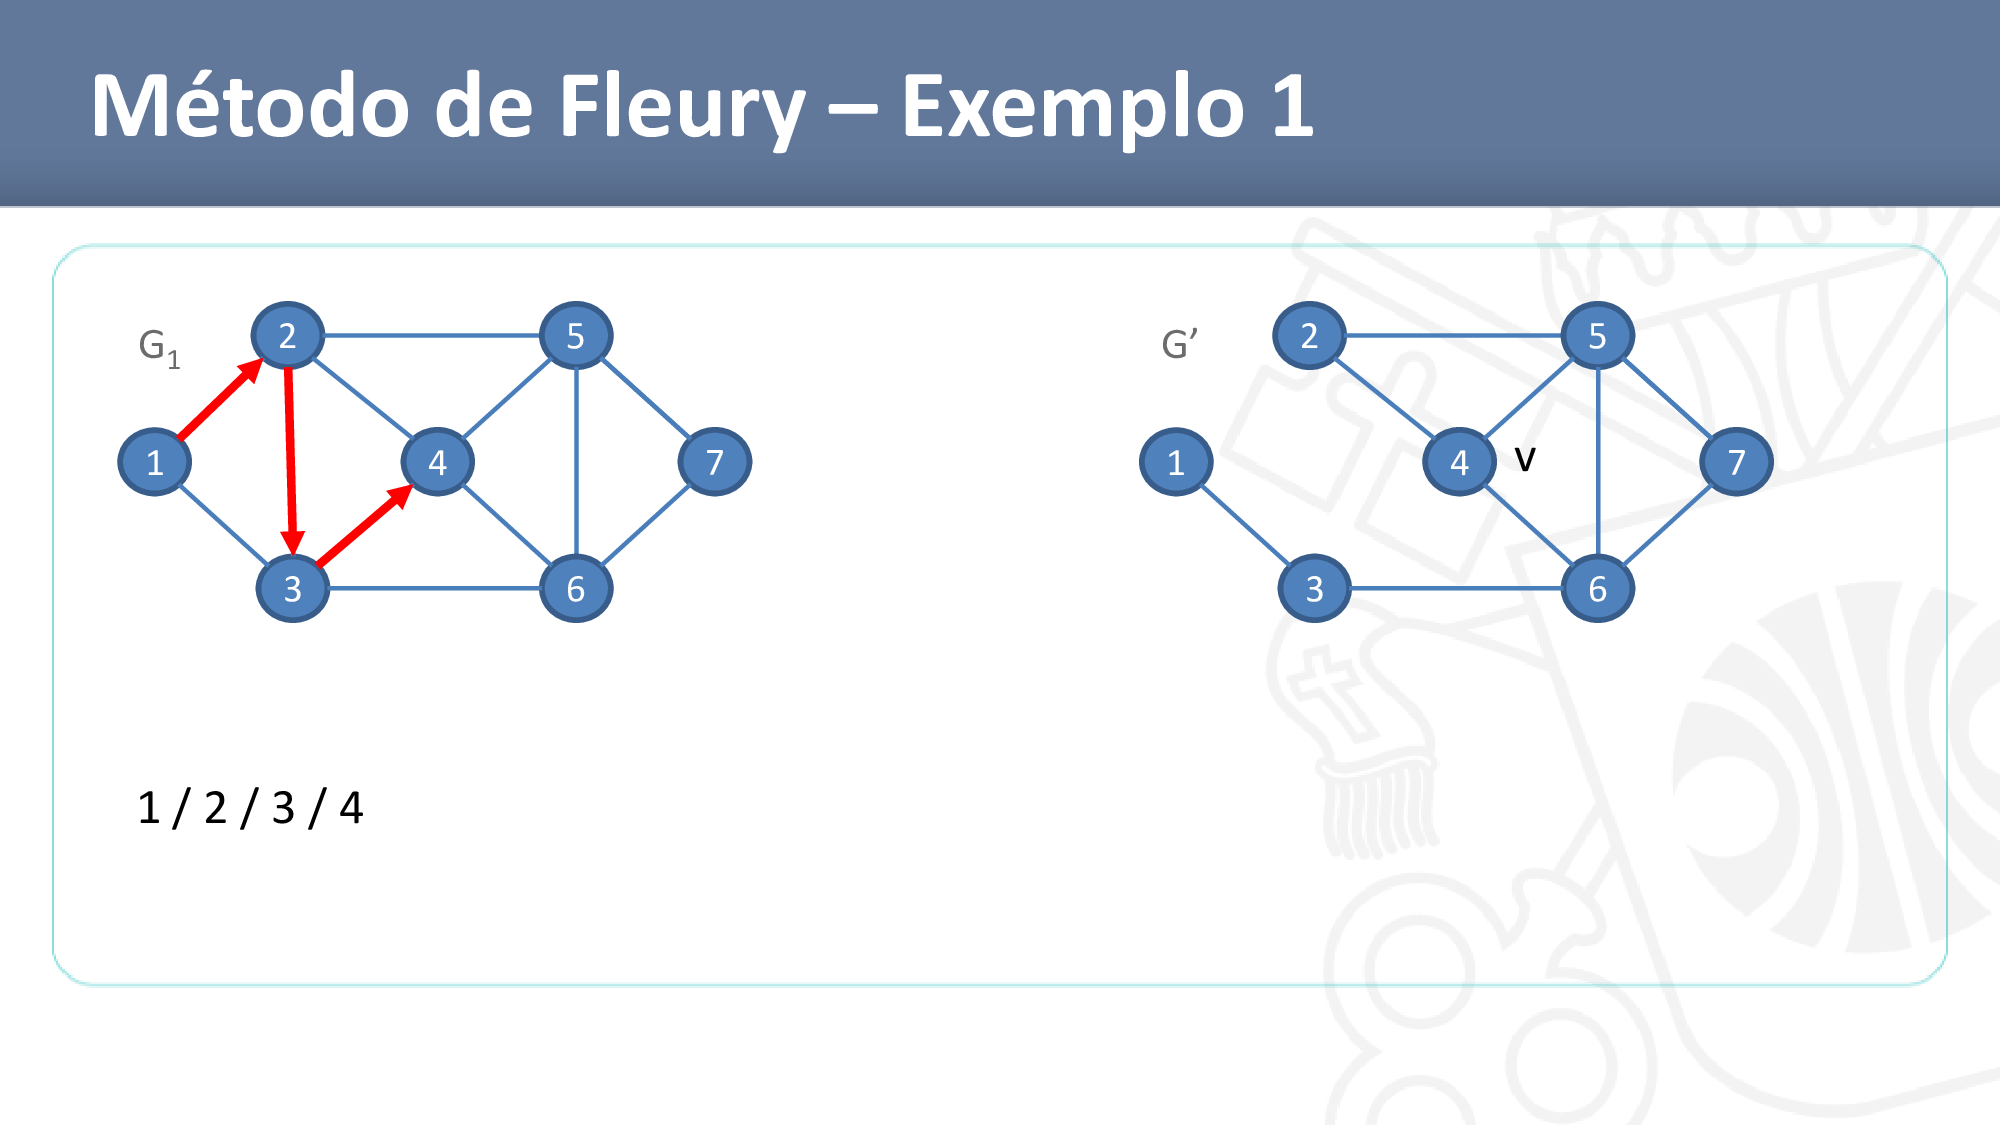
\includegraphics[width=\textwidth]{imagem/graficos/1a1455b7b9174768d1c6a0d41673e79dHTztESkzBtQzsXWu-31.png}
	\end{subfigure}
	\begin{subfigure}{.6\textwidth}
		\centering
		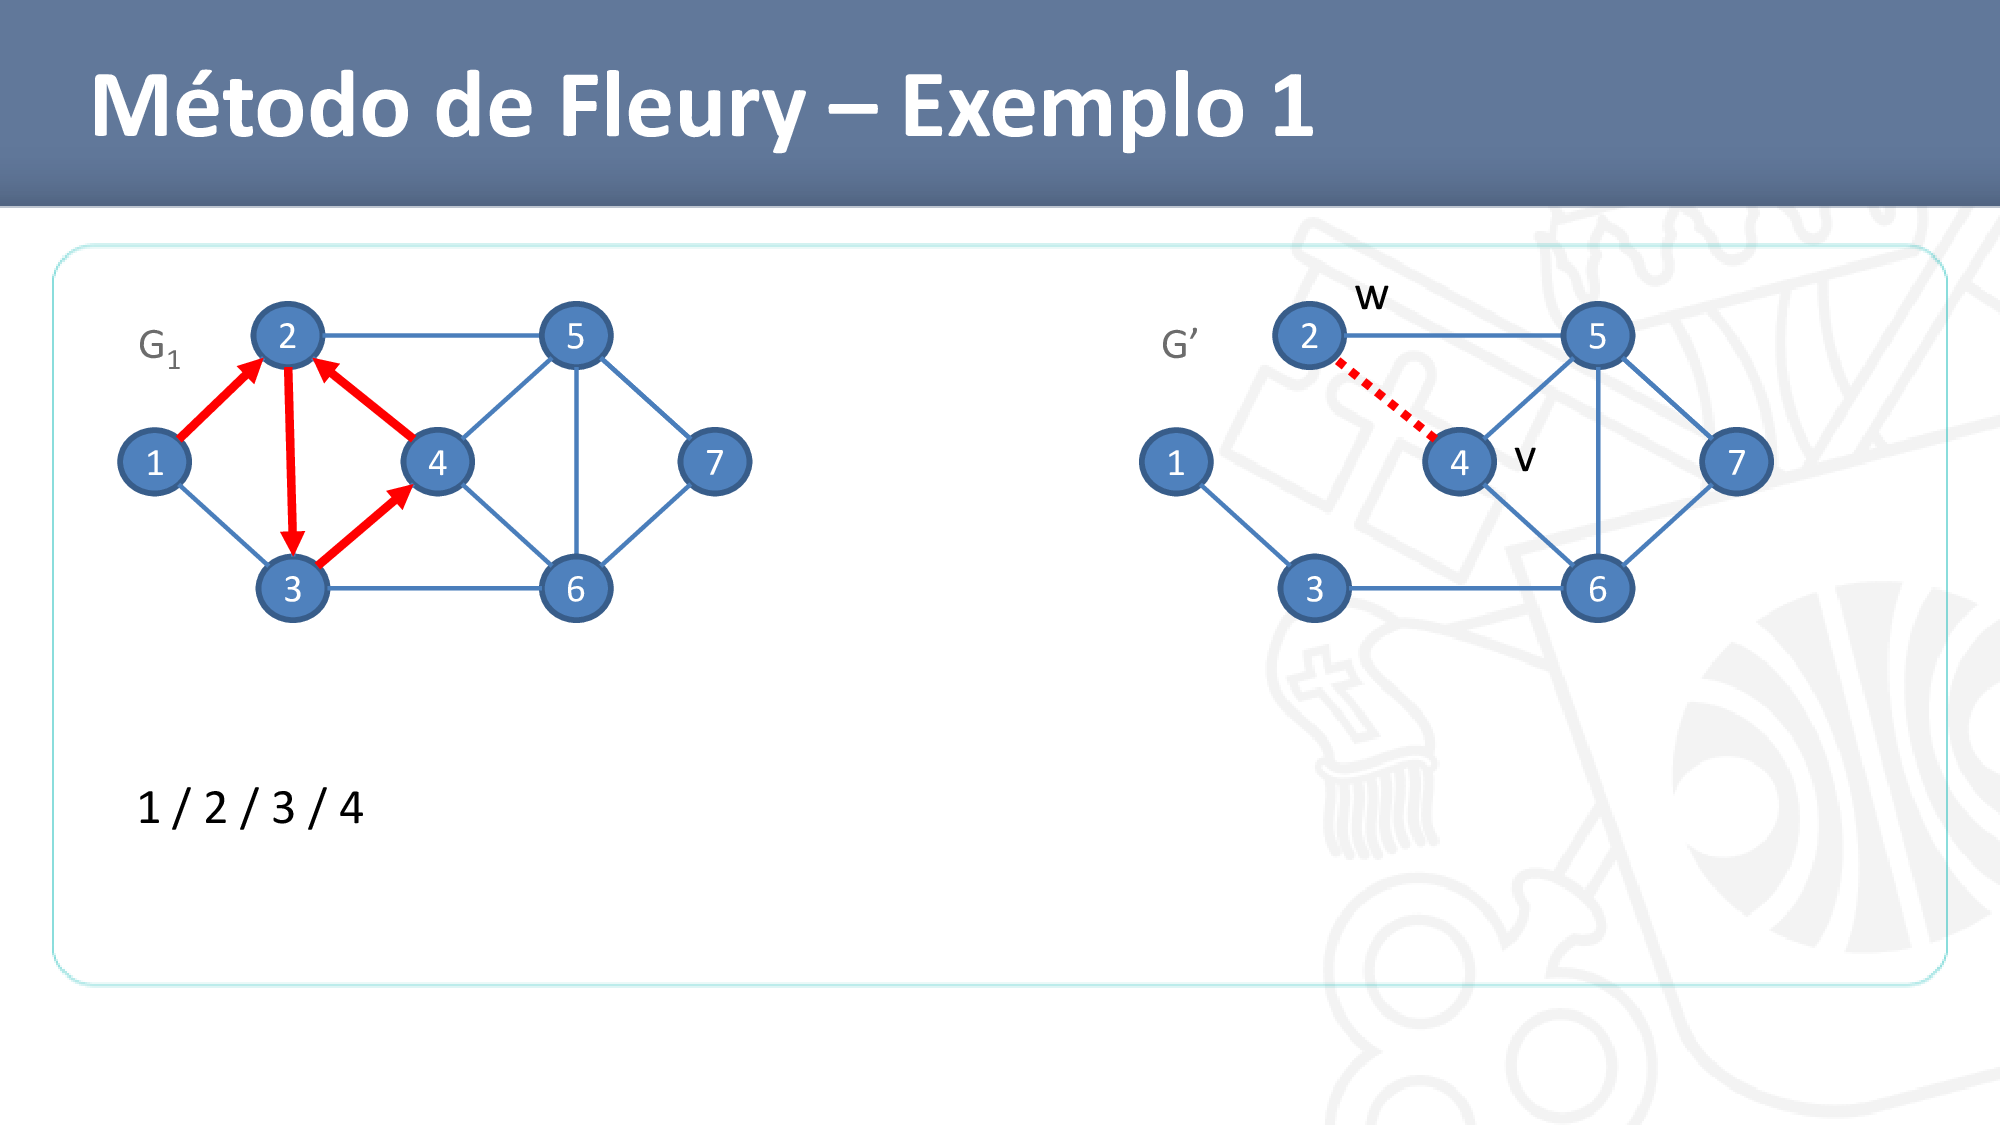
\includegraphics[width=\textwidth]{imagem/graficos/1a1455b7b9174768d1c6a0d41673e79dHTztESkzBtQzsXWu-32.png}
	\end{subfigure}
\end{figure}
\begin{figure}[H]
	\begin{subfigure}{.6\textwidth}
		\centering
		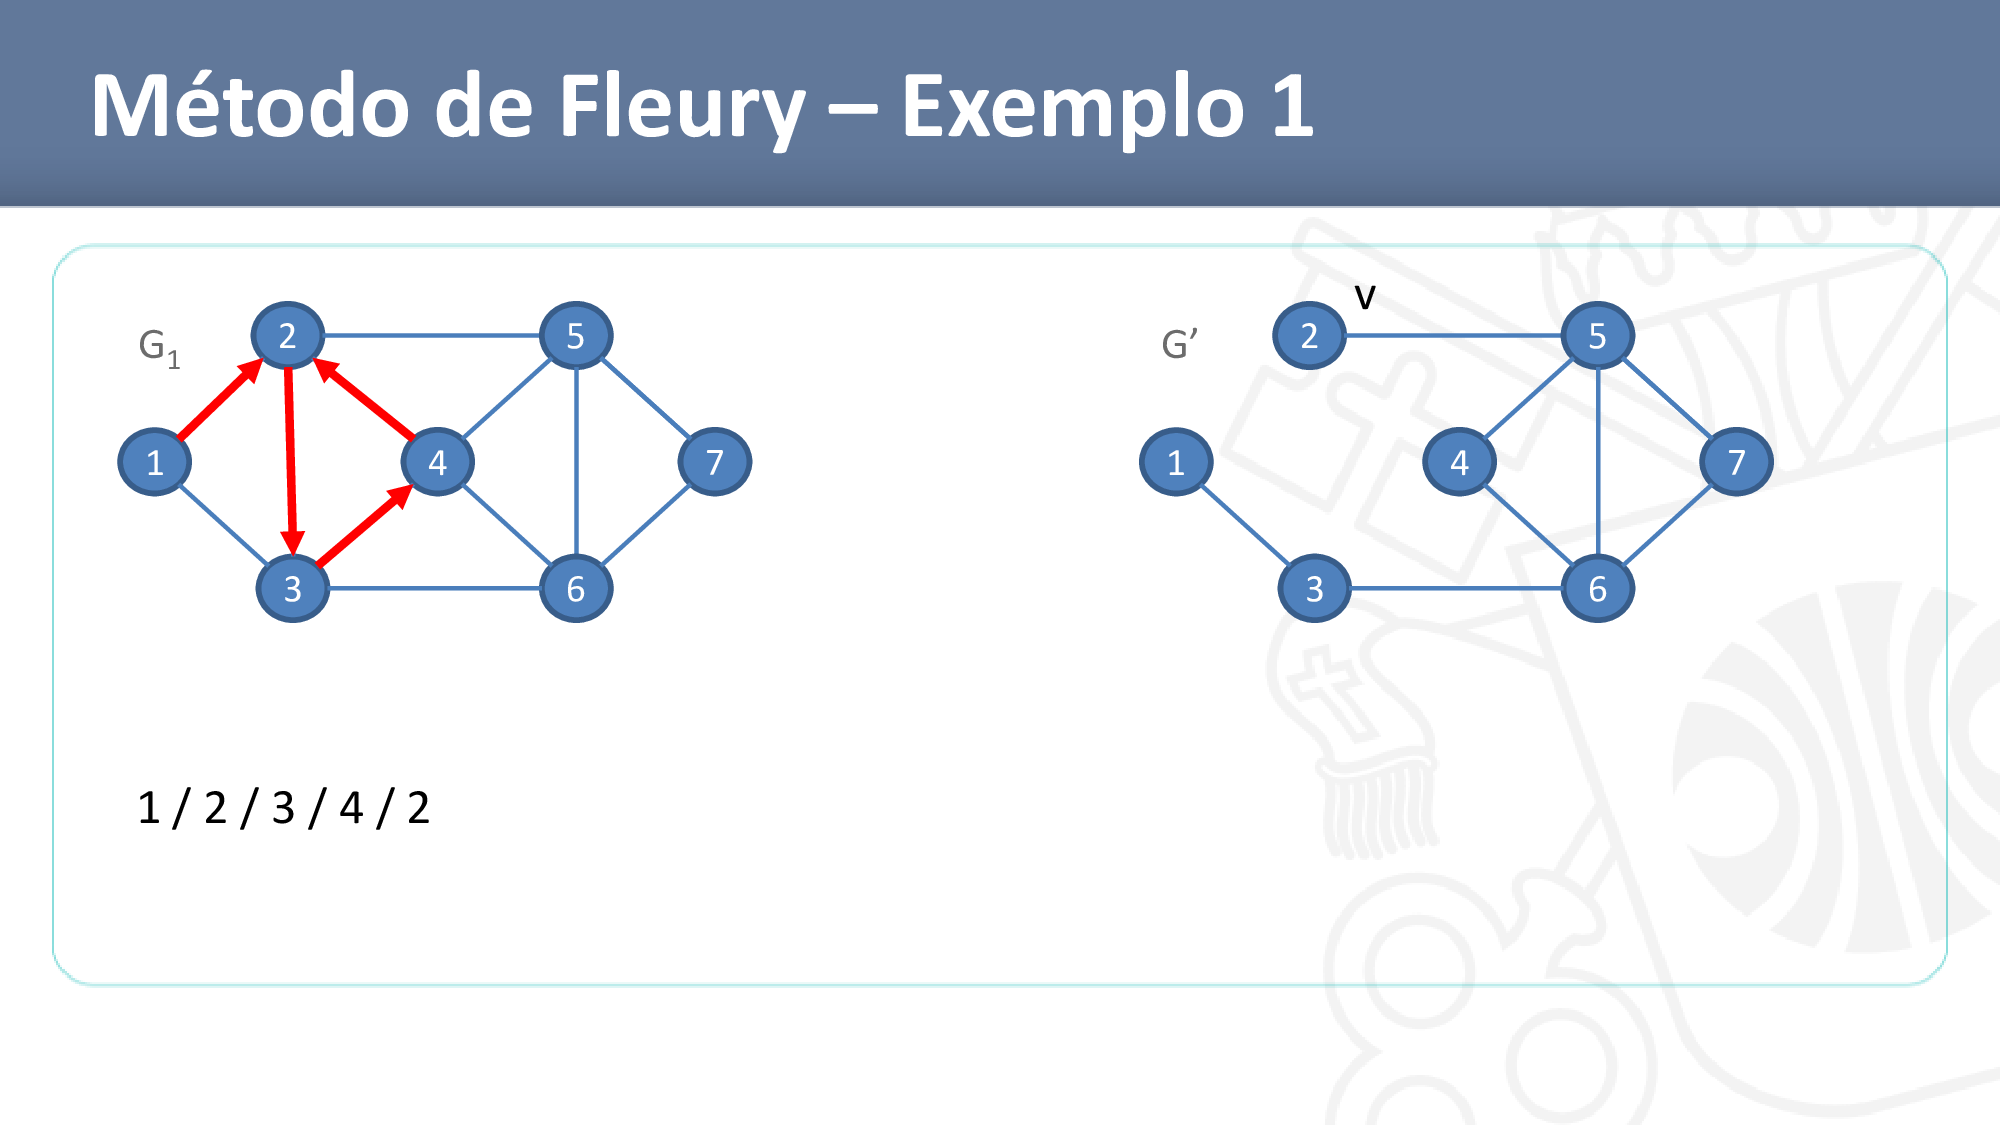
\includegraphics[width=\textwidth]{imagem/graficos/1a1455b7b9174768d1c6a0d41673e79dHTztESkzBtQzsXWu-33.png}
	\end{subfigure}
	\begin{subfigure}{.6\textwidth}
		\centering
		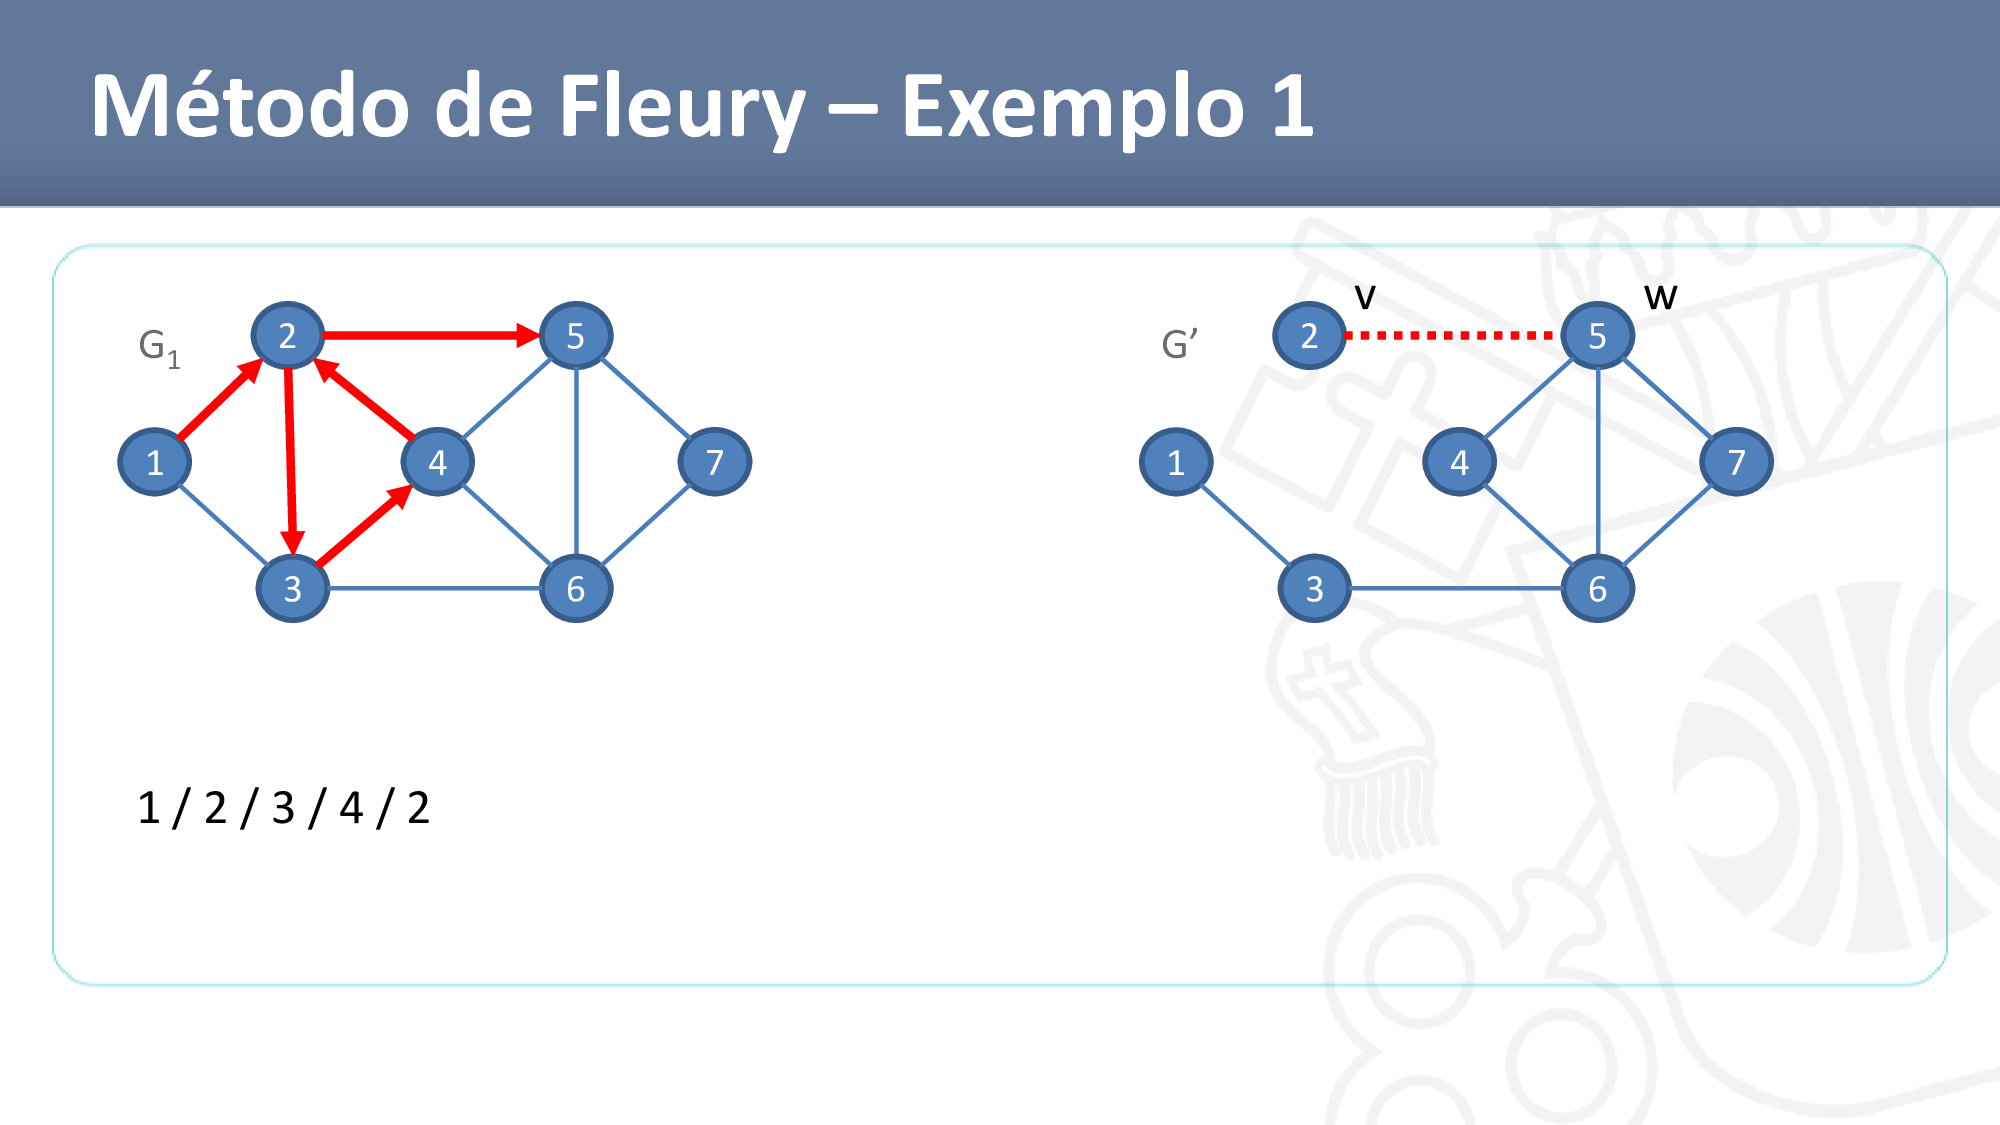
\includegraphics[width=\textwidth]{imagem/graficos/1a1455b7b9174768d1c6a0d41673e79dHTztESkzBtQzsXWu-34.png}
	\end{subfigure}
\end{figure}
\begin{figure}[H]
	\begin{subfigure}{.6\textwidth}
		\centering
		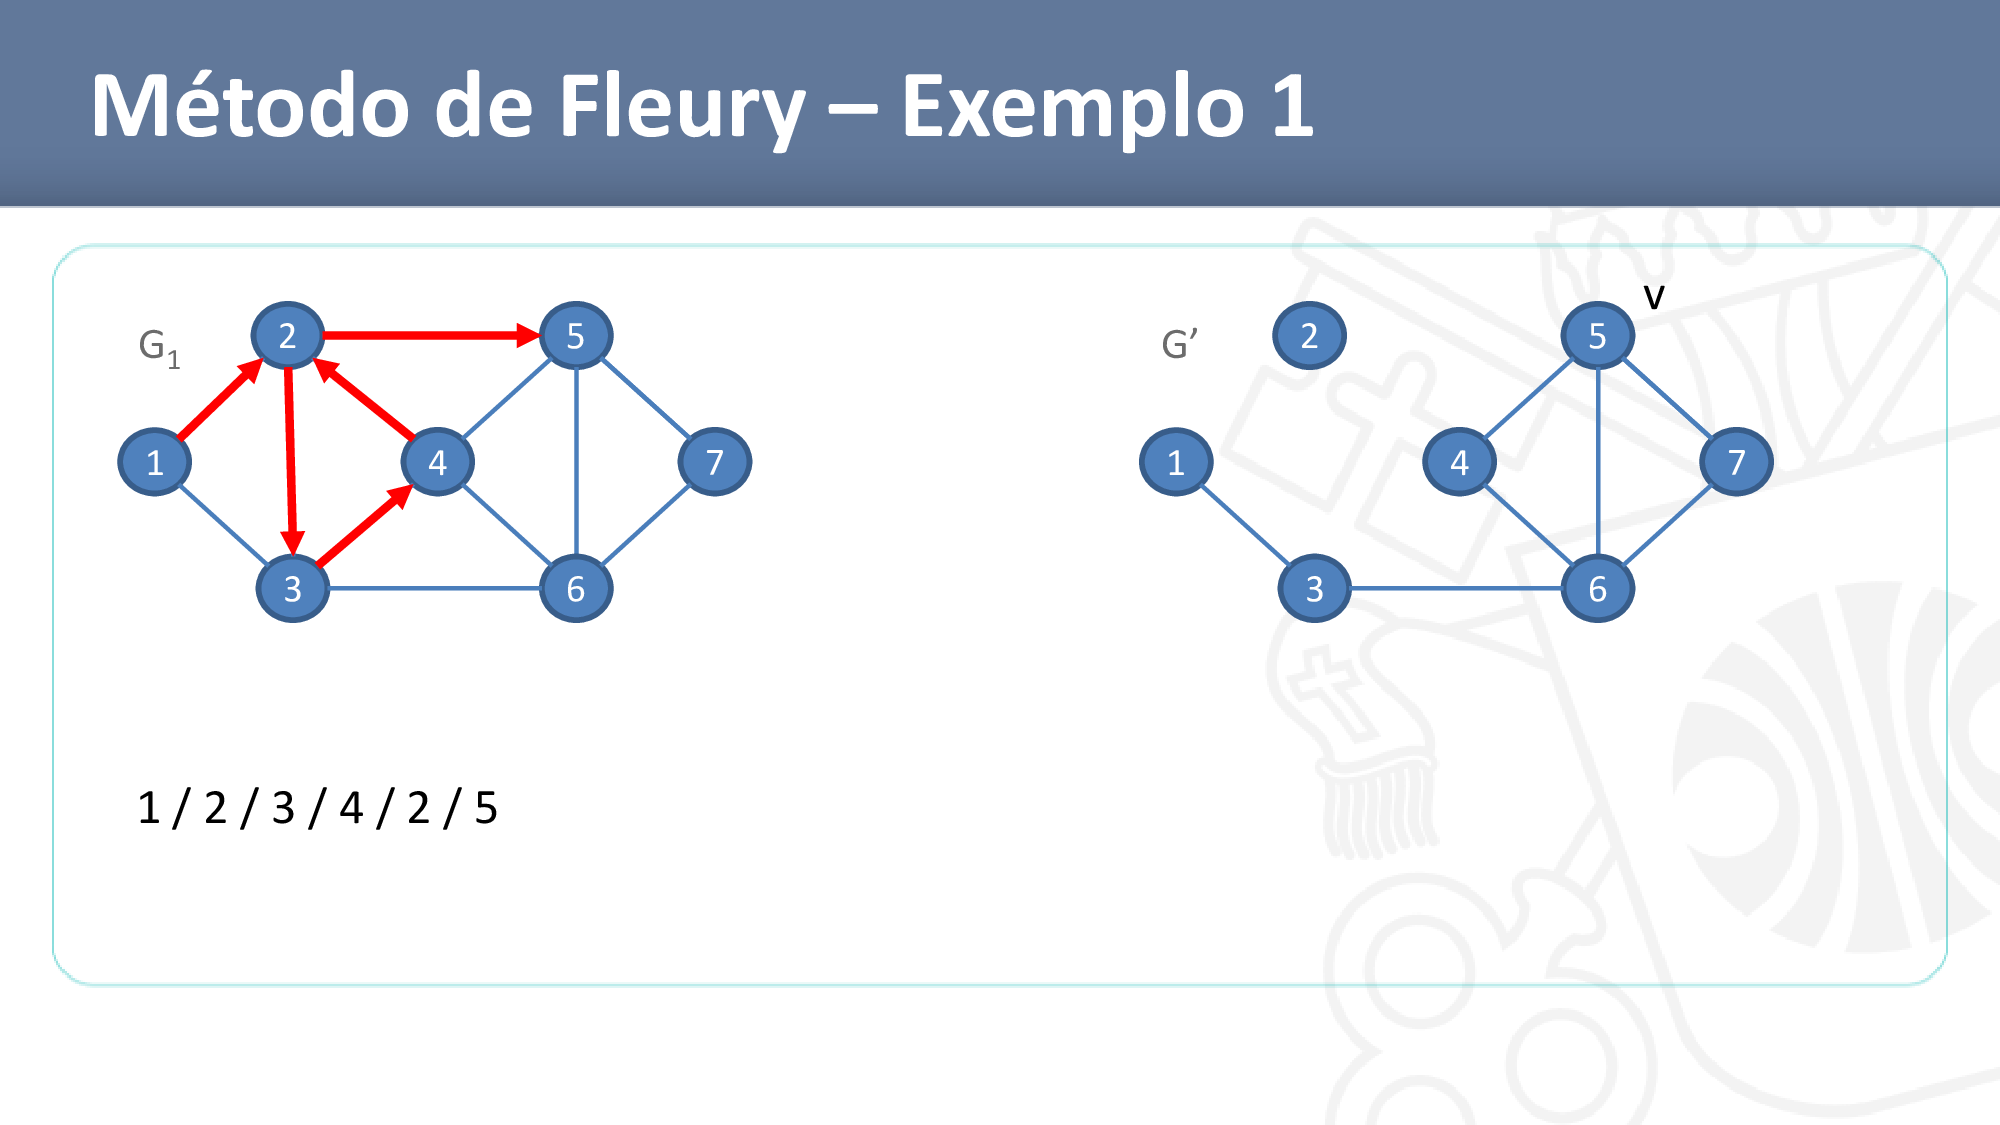
\includegraphics[width=\textwidth]{imagem/graficos/1a1455b7b9174768d1c6a0d41673e79dHTztESkzBtQzsXWu-35.png}
	\end{subfigure}
	\begin{subfigure}{.6\textwidth}
		\centering
		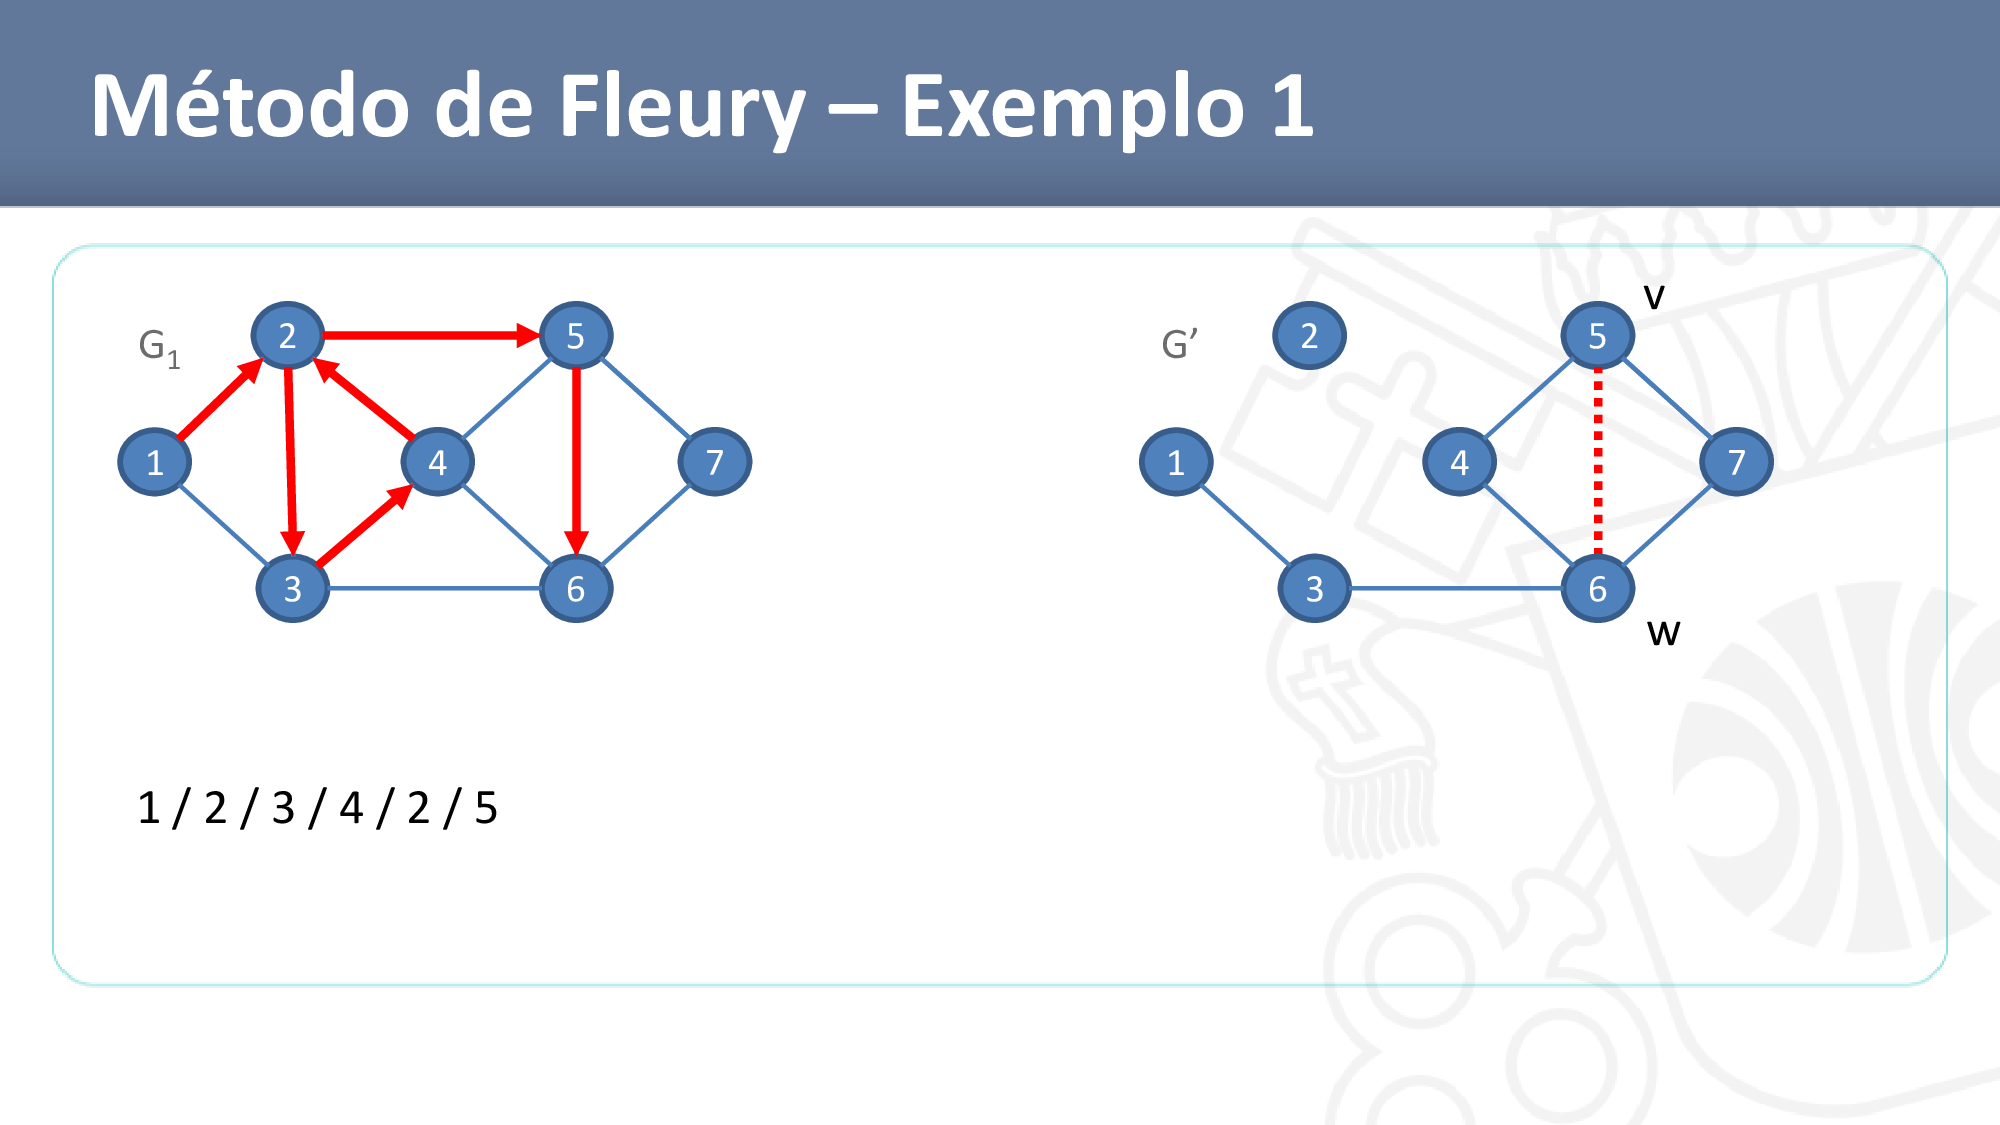
\includegraphics[width=\textwidth]{imagem/graficos/1a1455b7b9174768d1c6a0d41673e79dHTztESkzBtQzsXWu-36.png}
	\end{subfigure}
\end{figure}
\begin{figure}[H]
	\begin{subfigure}{.6\textwidth}
		\centering
		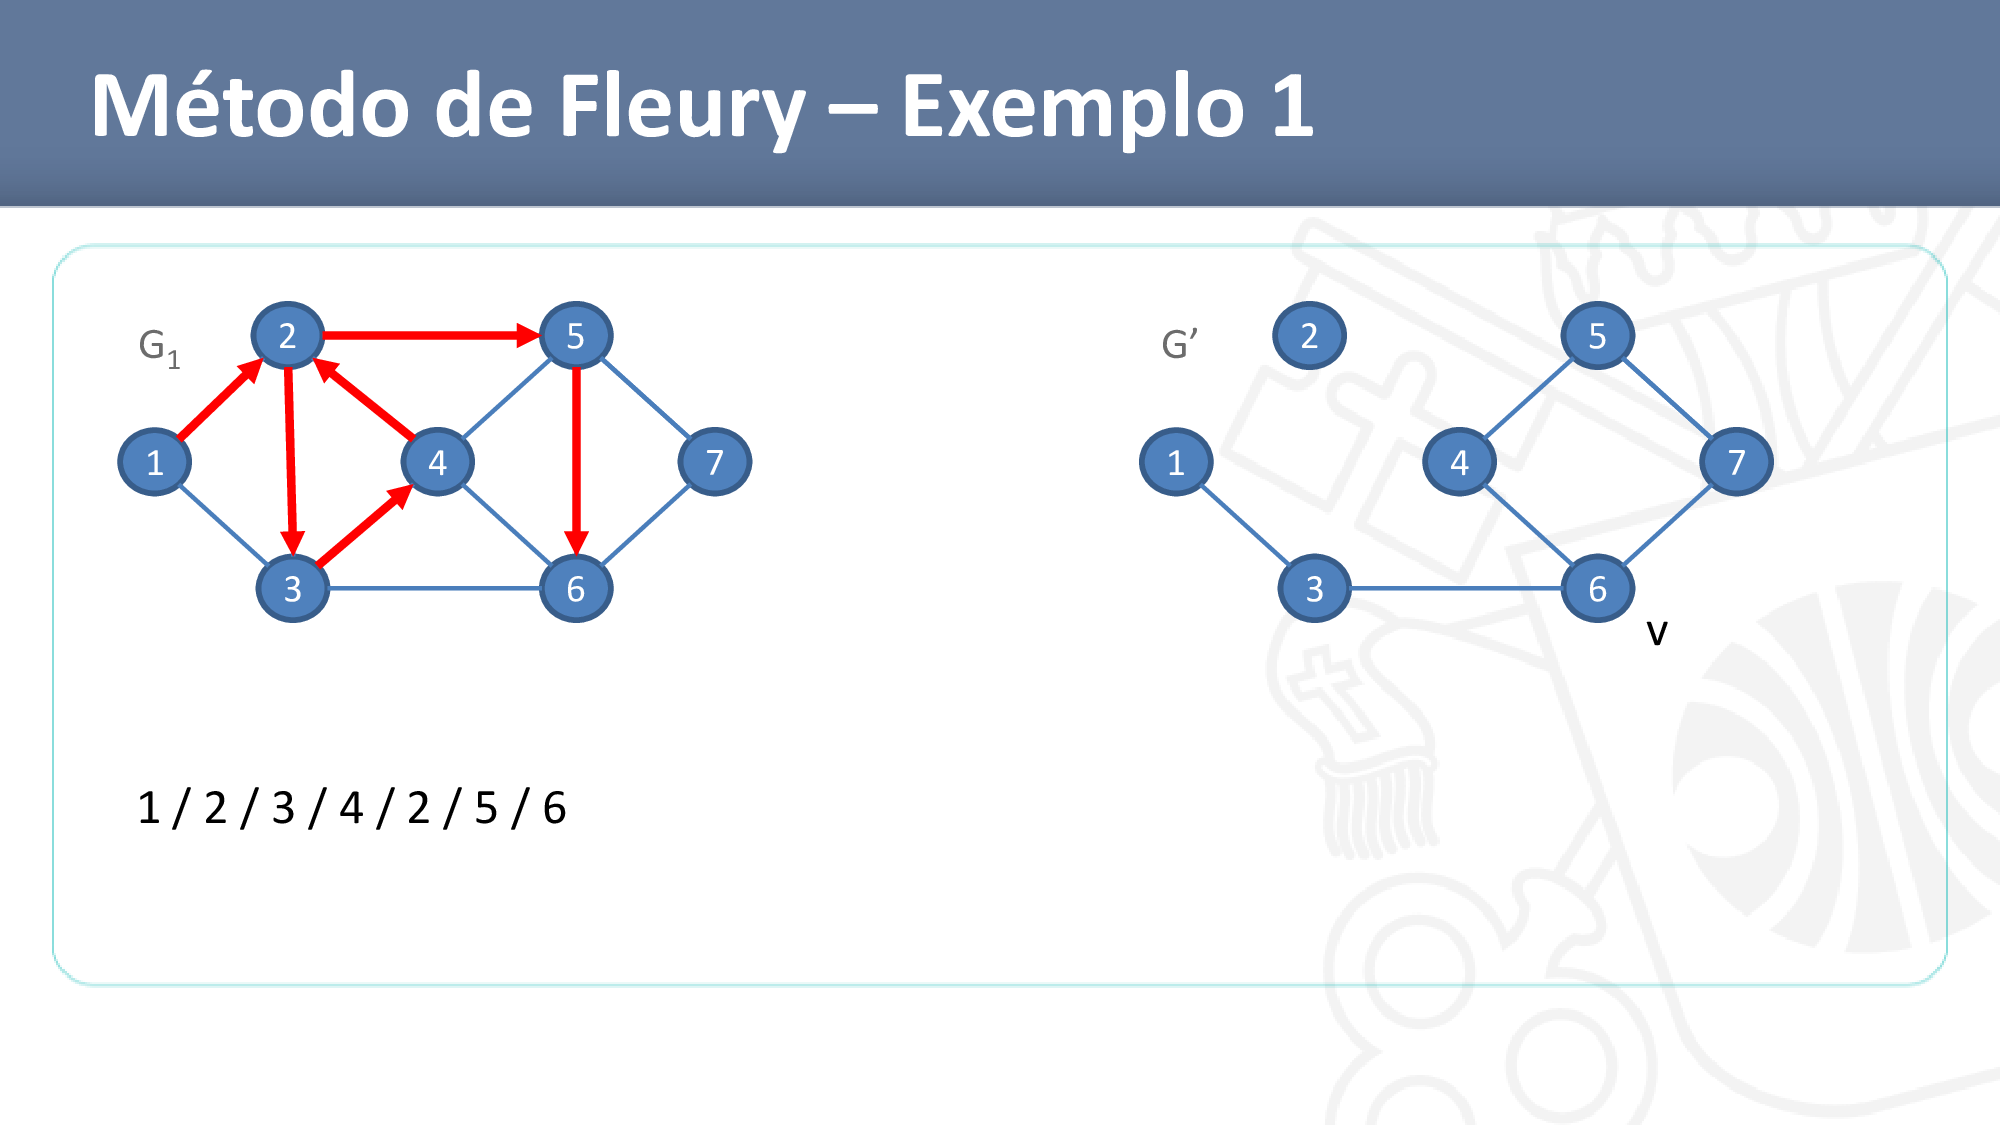
\includegraphics[width=\textwidth]{imagem/graficos/1a1455b7b9174768d1c6a0d41673e79dHTztESkzBtQzsXWu-37.png}
	\end{subfigure}
	\begin{subfigure}{.6\textwidth}
		\centering
		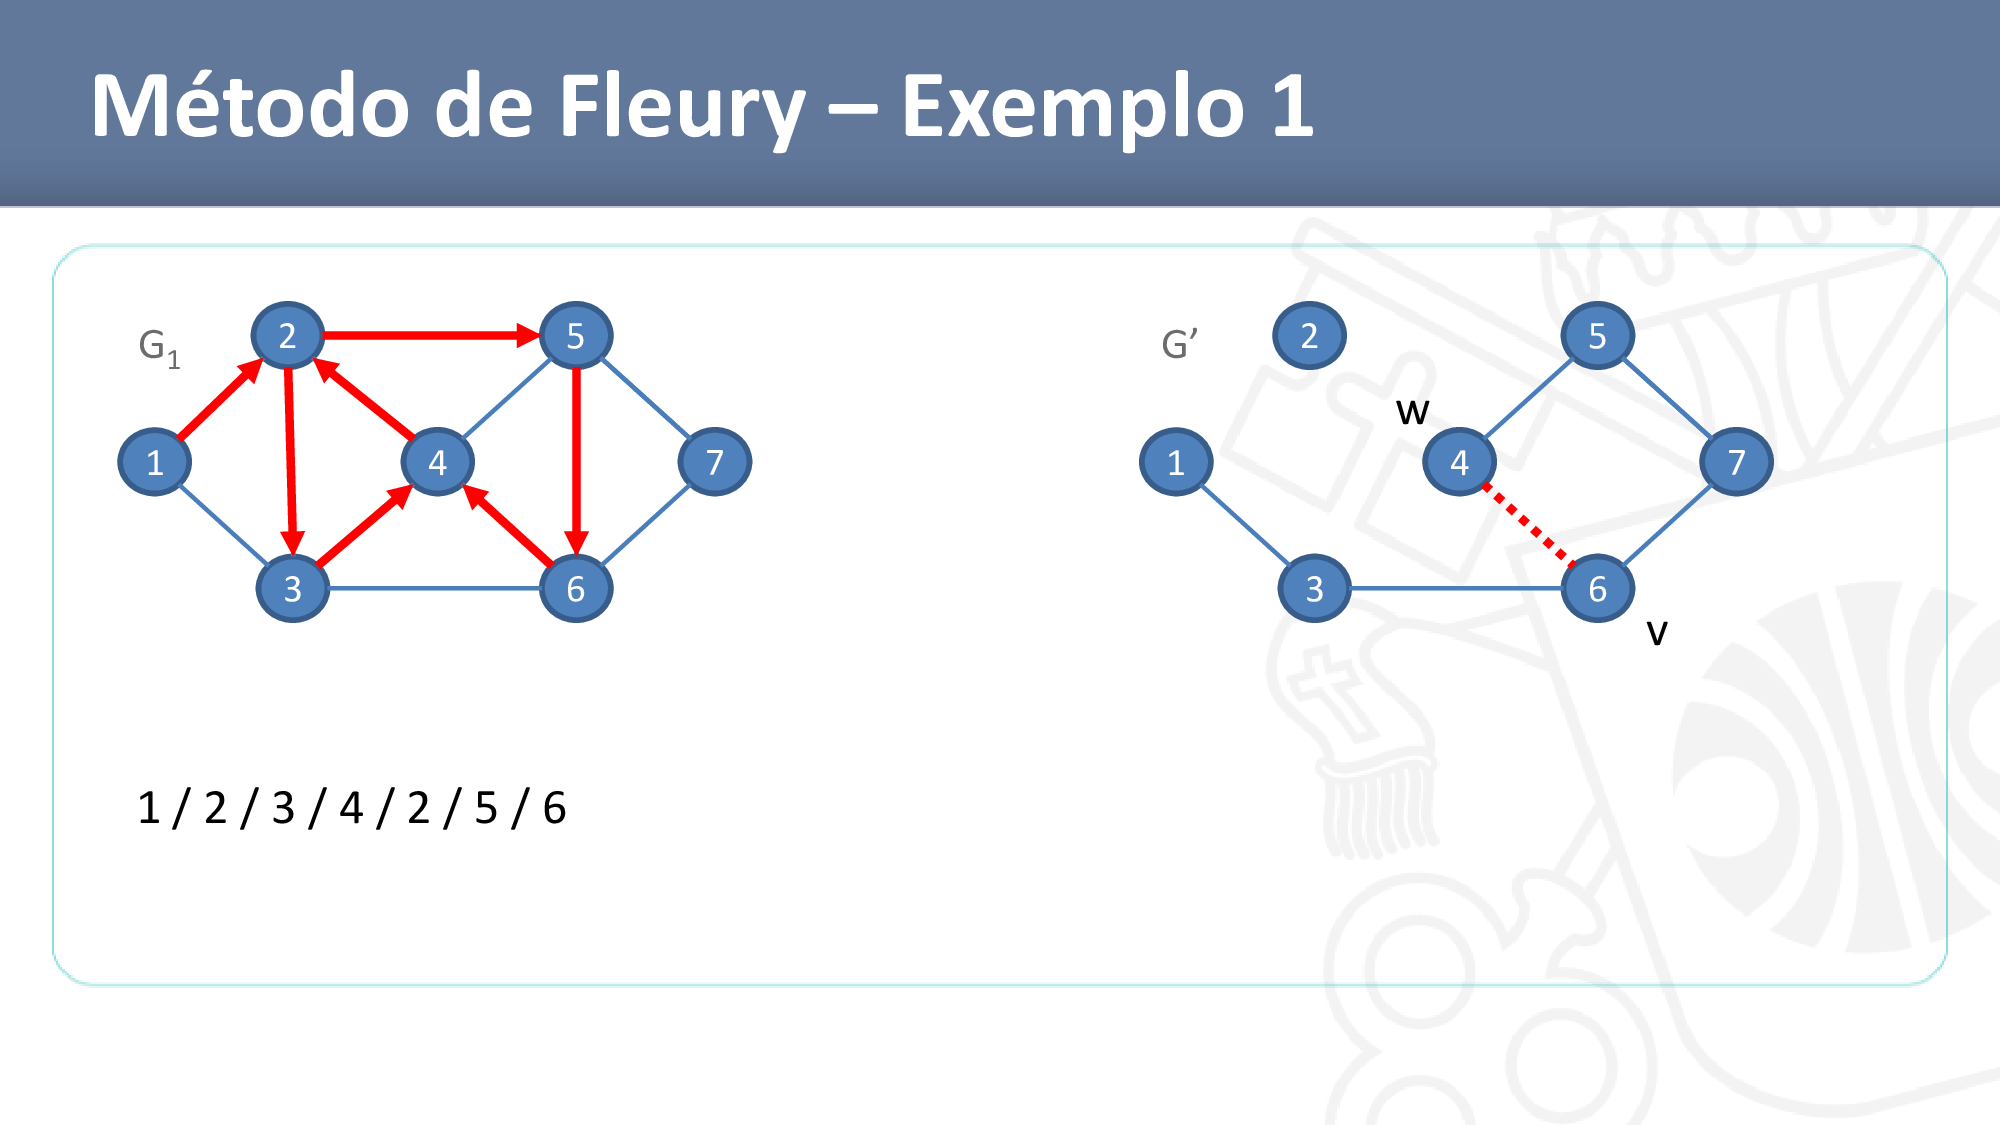
\includegraphics[width=\textwidth]{imagem/graficos/1a1455b7b9174768d1c6a0d41673e79dHTztESkzBtQzsXWu-38.png}
	\end{subfigure}
\end{figure}
\begin{figure}[H]
	\begin{subfigure}{.6\textwidth}
		\centering
		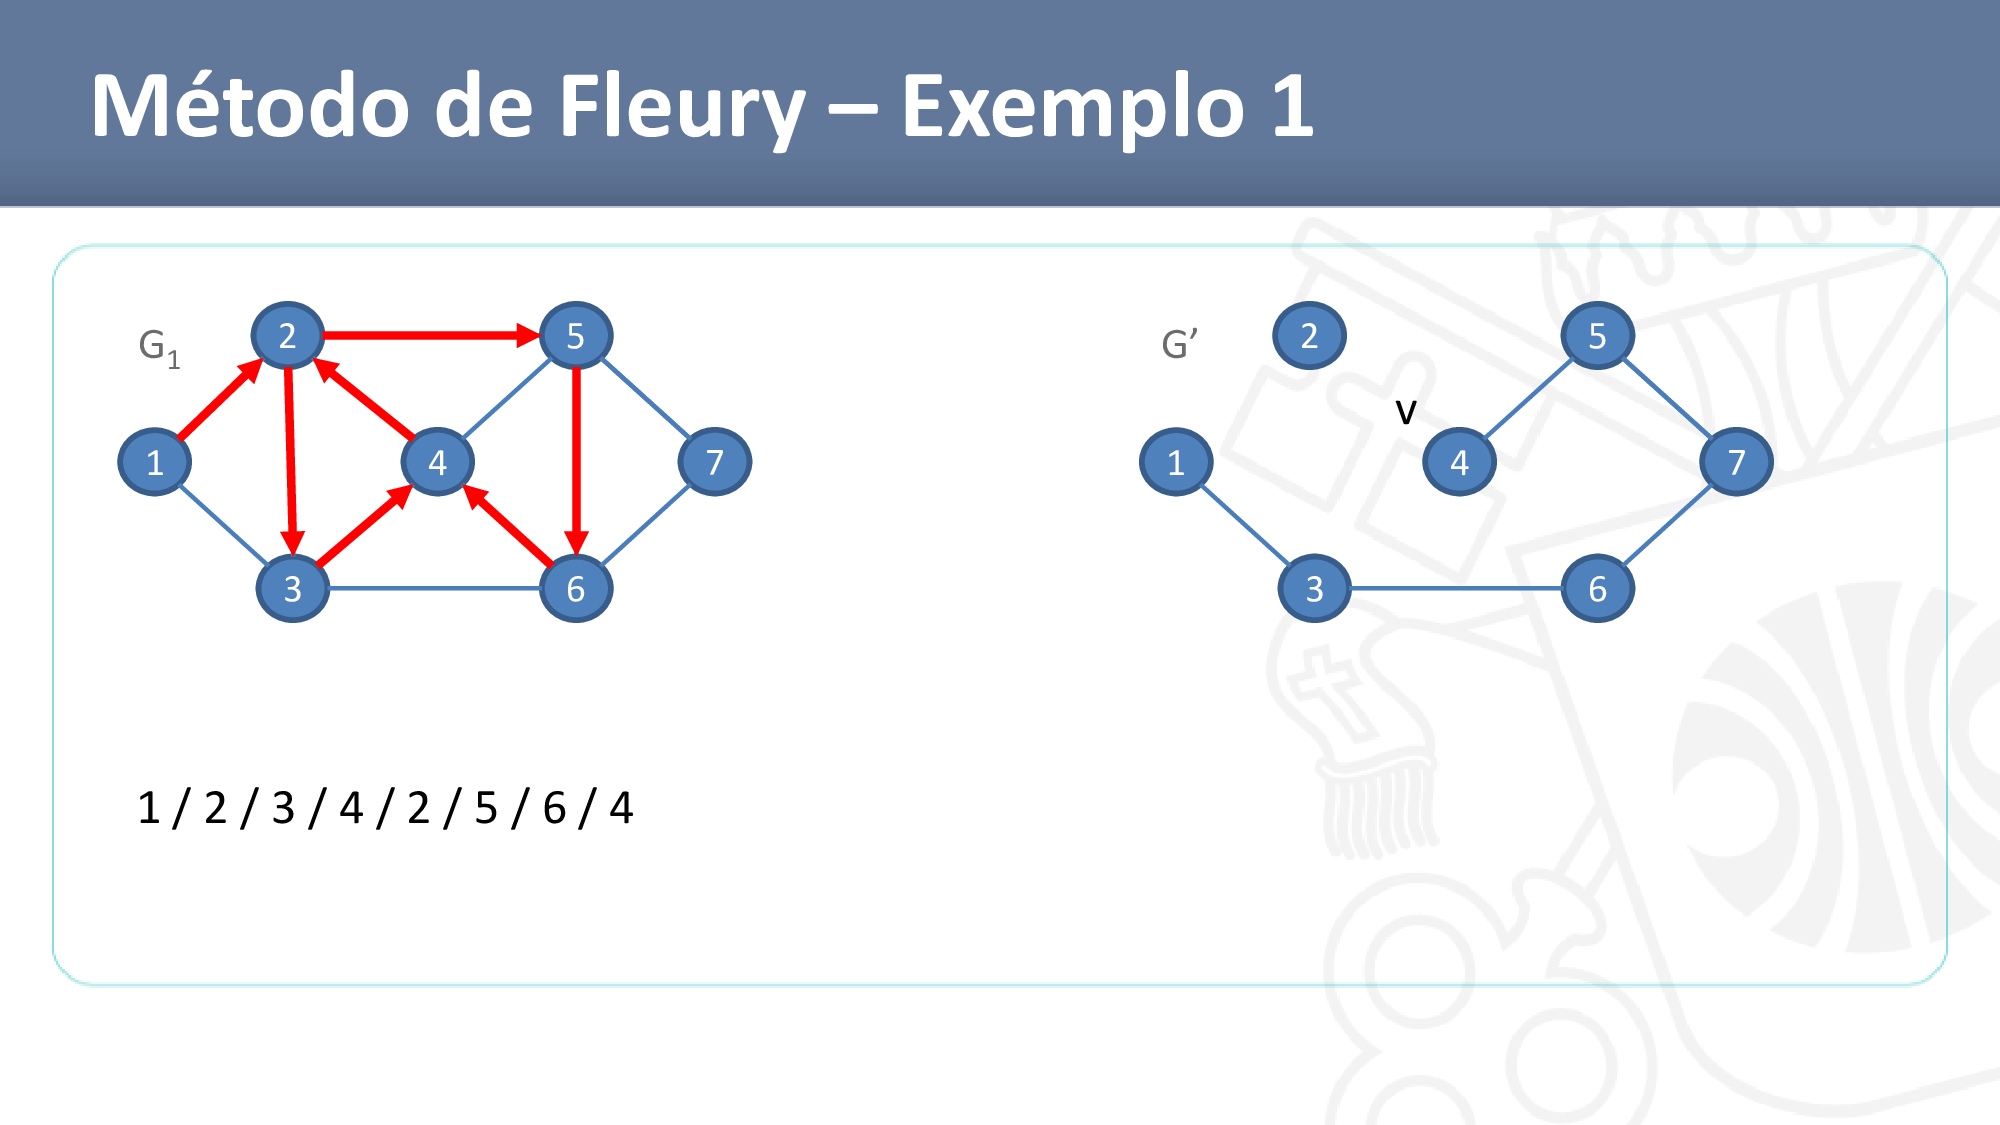
\includegraphics[width=\textwidth]{imagem/graficos/1a1455b7b9174768d1c6a0d41673e79dHTztESkzBtQzsXWu-39.png}
	\end{subfigure}
	\begin{subfigure}{.6\textwidth}
		\centering
		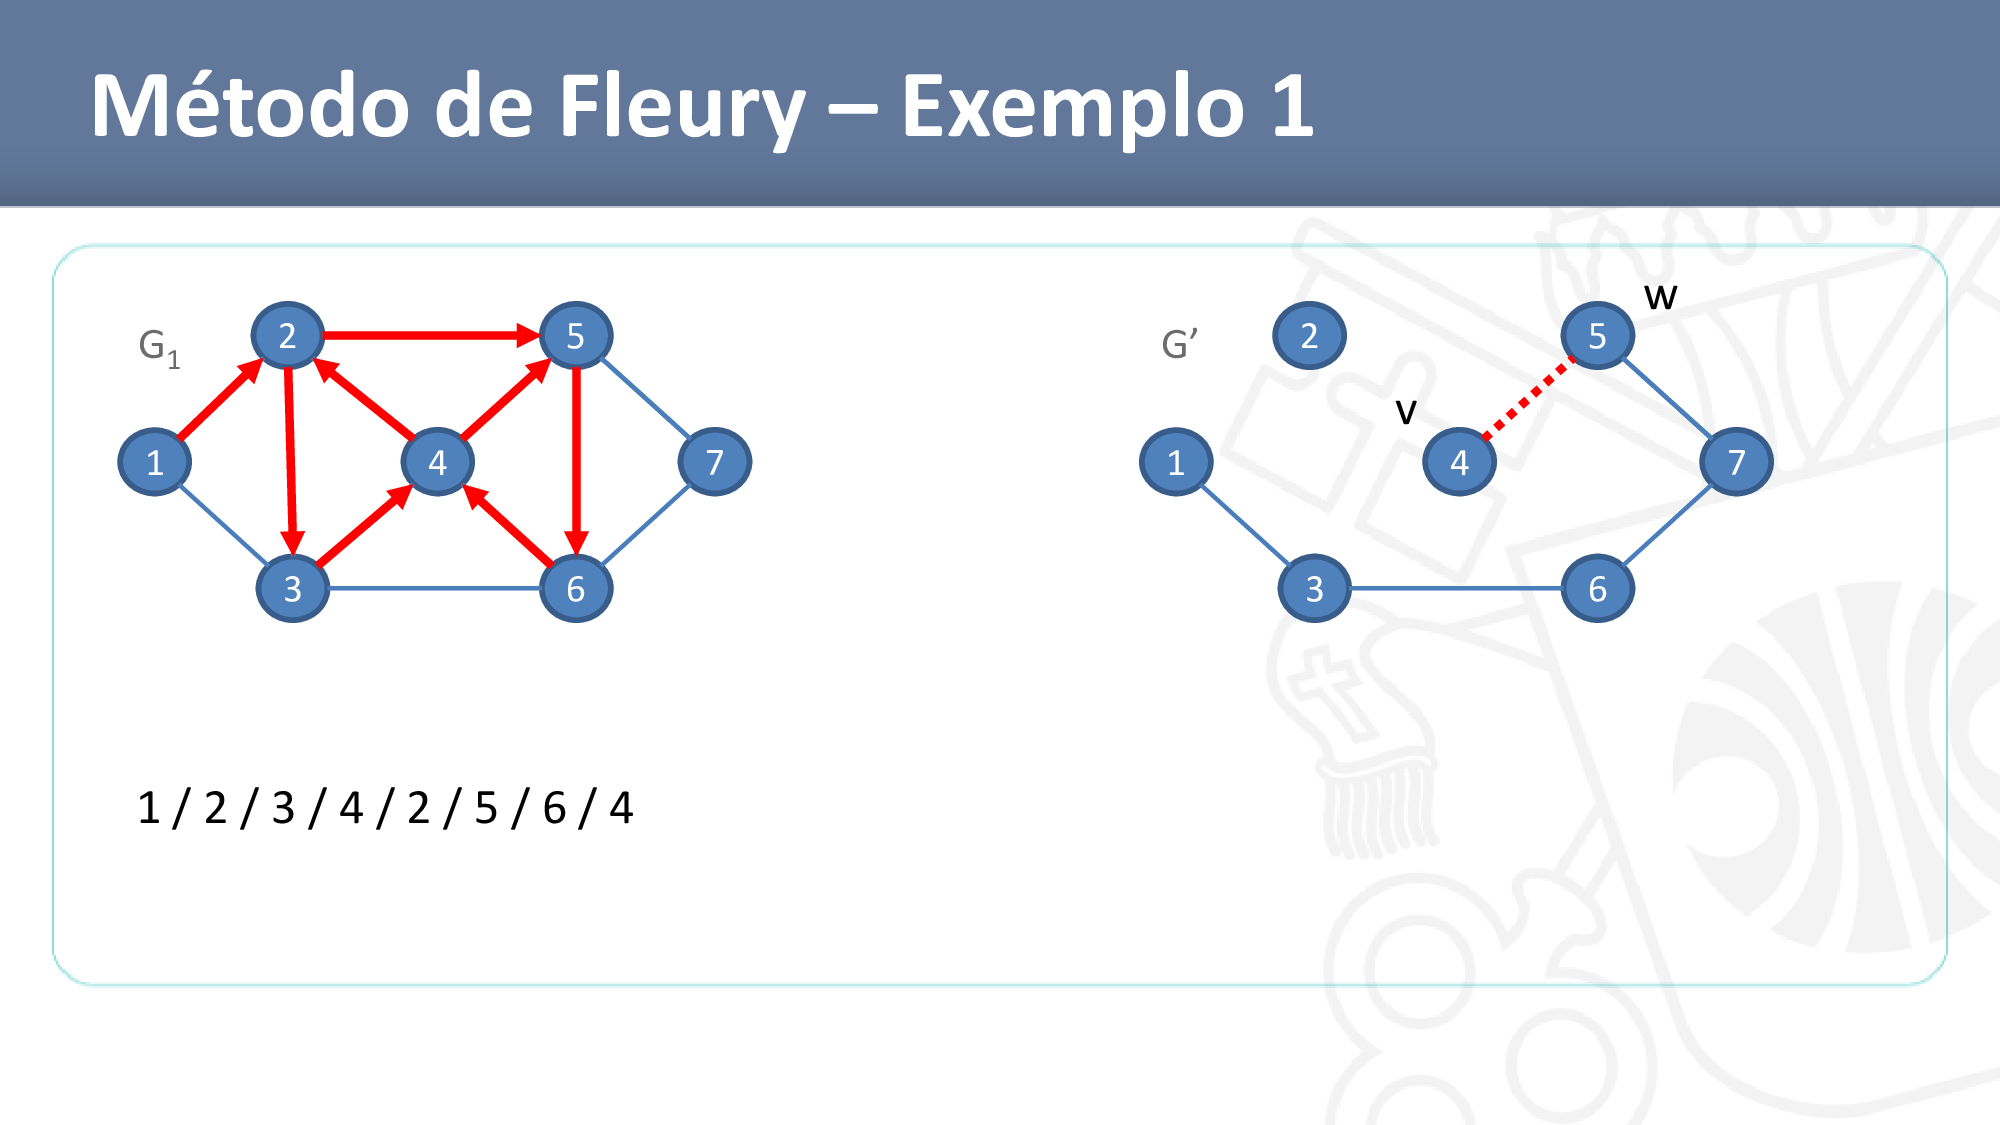
\includegraphics[width=\textwidth]{imagem/graficos/1a1455b7b9174768d1c6a0d41673e79dHTztESkzBtQzsXWu-40.png}
	\end{subfigure}
\end{figure}
\begin{figure}[H]
	\begin{subfigure}{.6\textwidth}
		\centering
		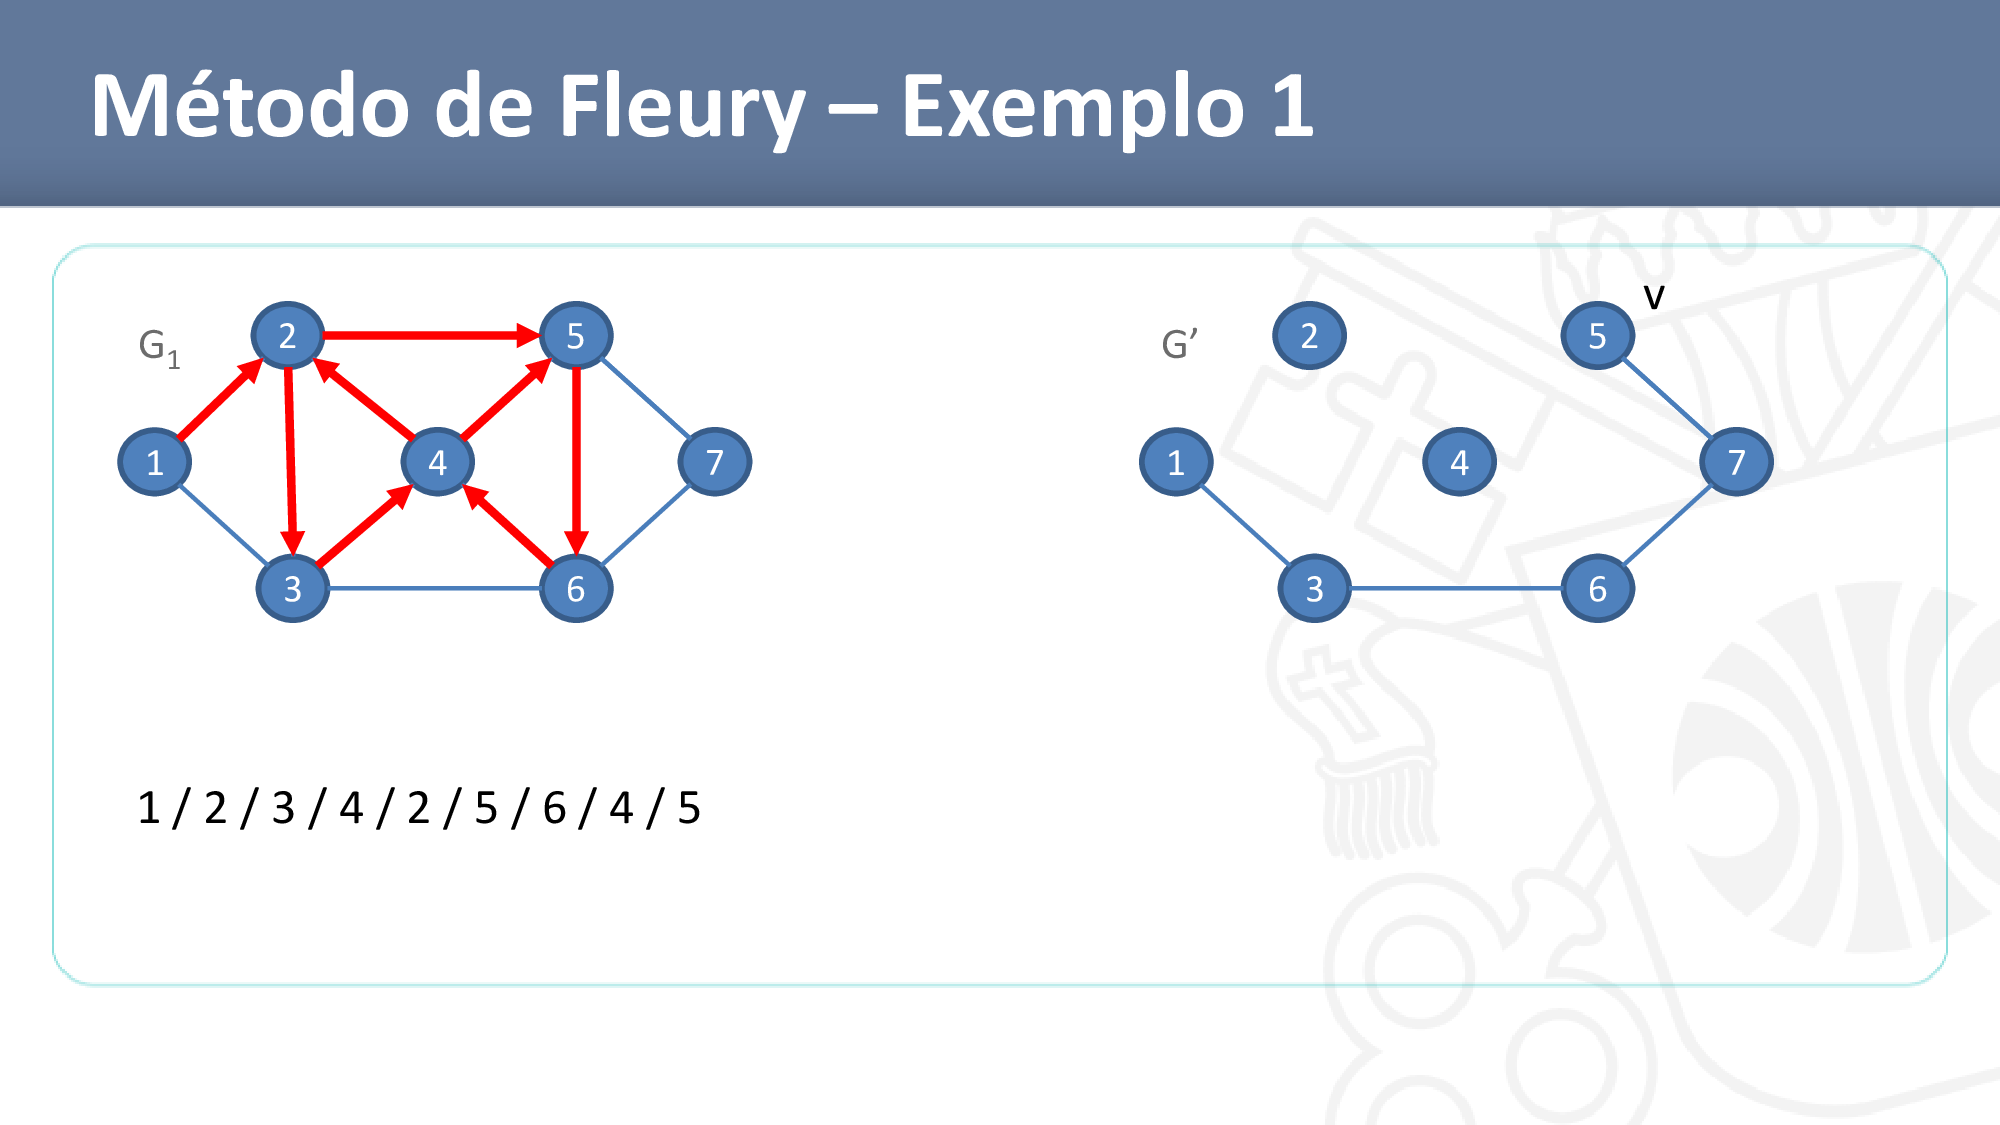
\includegraphics[width=\textwidth]{imagem/graficos/1a1455b7b9174768d1c6a0d41673e79dHTztESkzBtQzsXWu-41.png}
	\end{subfigure}
	\begin{subfigure}{.6\textwidth}
		\centering
		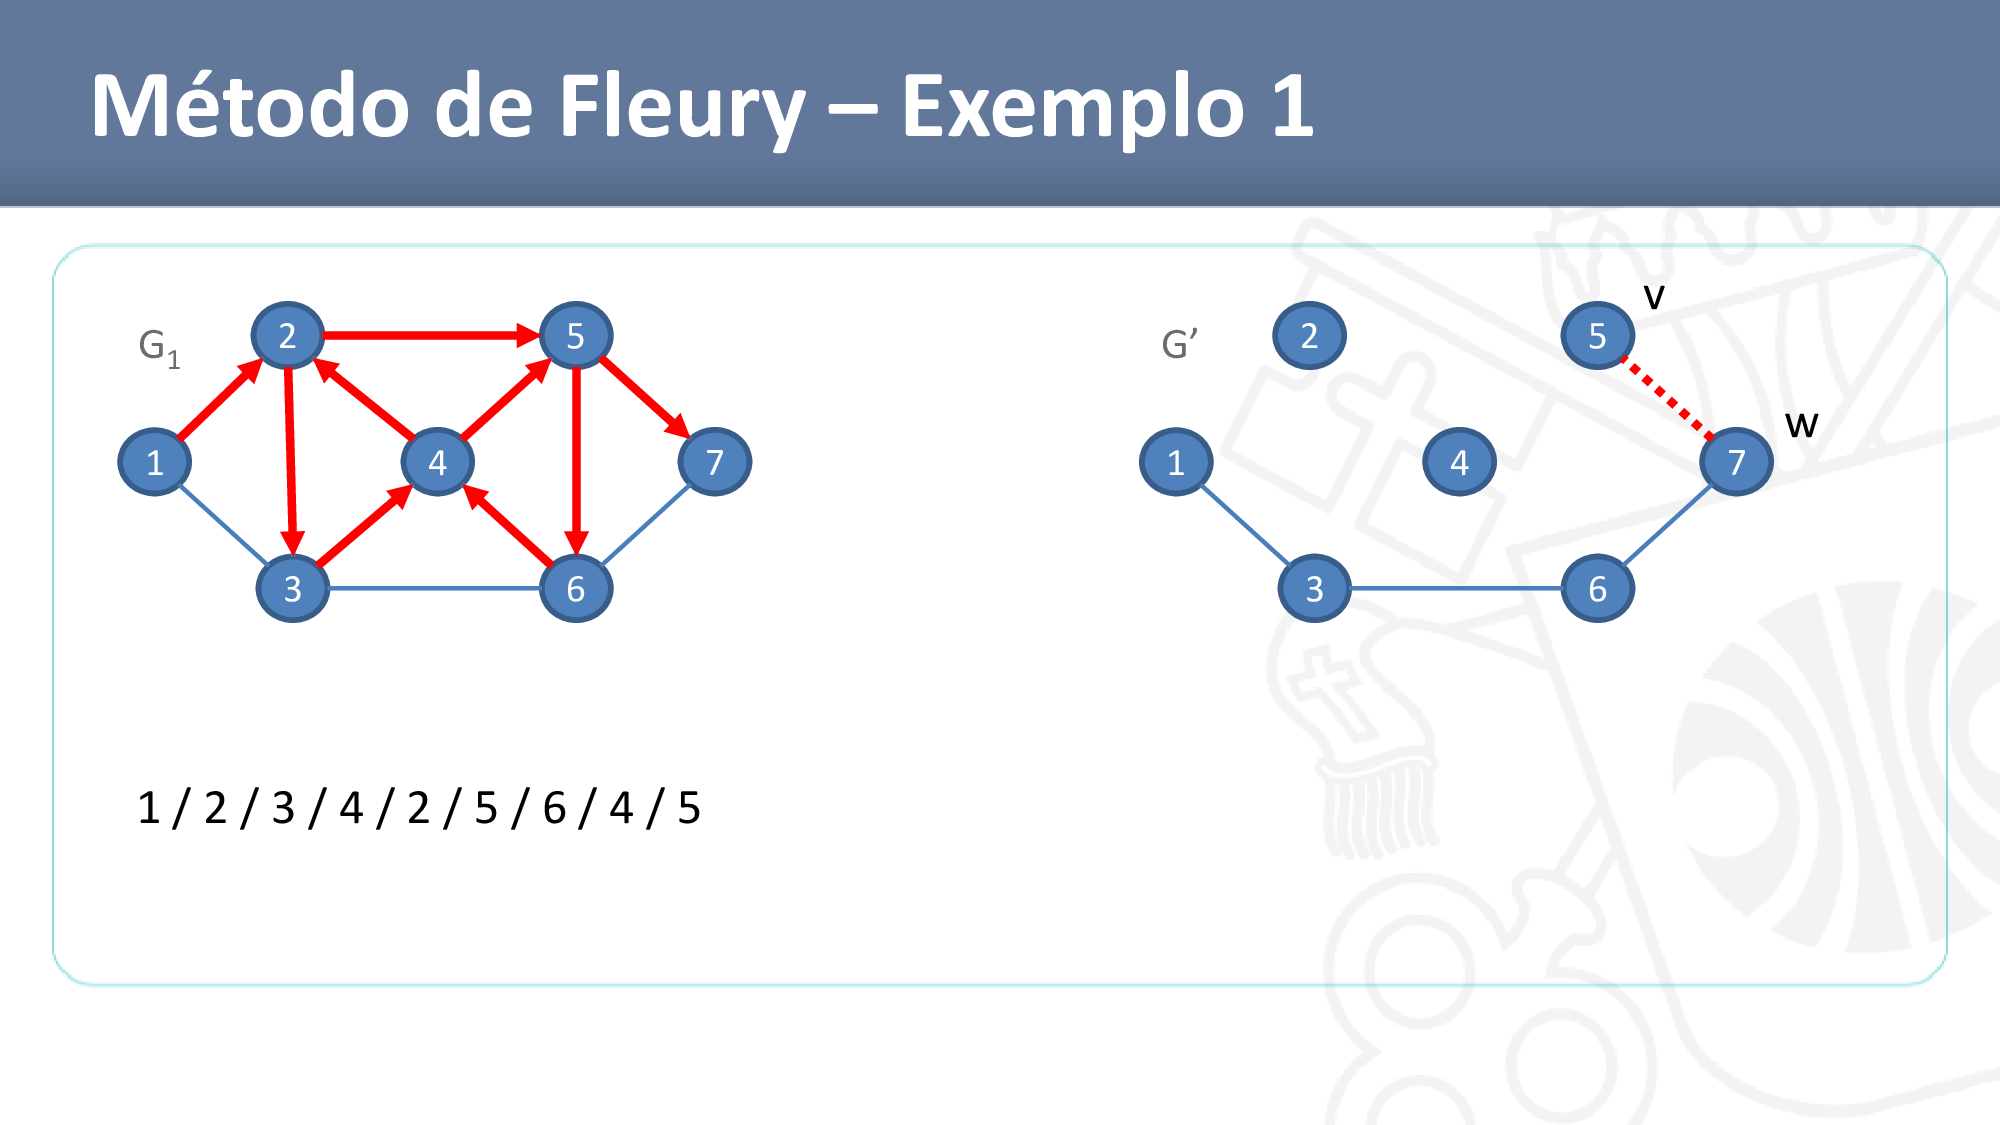
\includegraphics[width=\textwidth]{imagem/graficos/1a1455b7b9174768d1c6a0d41673e79dHTztESkzBtQzsXWu-42.png}
	\end{subfigure}
\end{figure}
\begin{figure}[H]
	\begin{subfigure}{.6\textwidth}
		\centering
		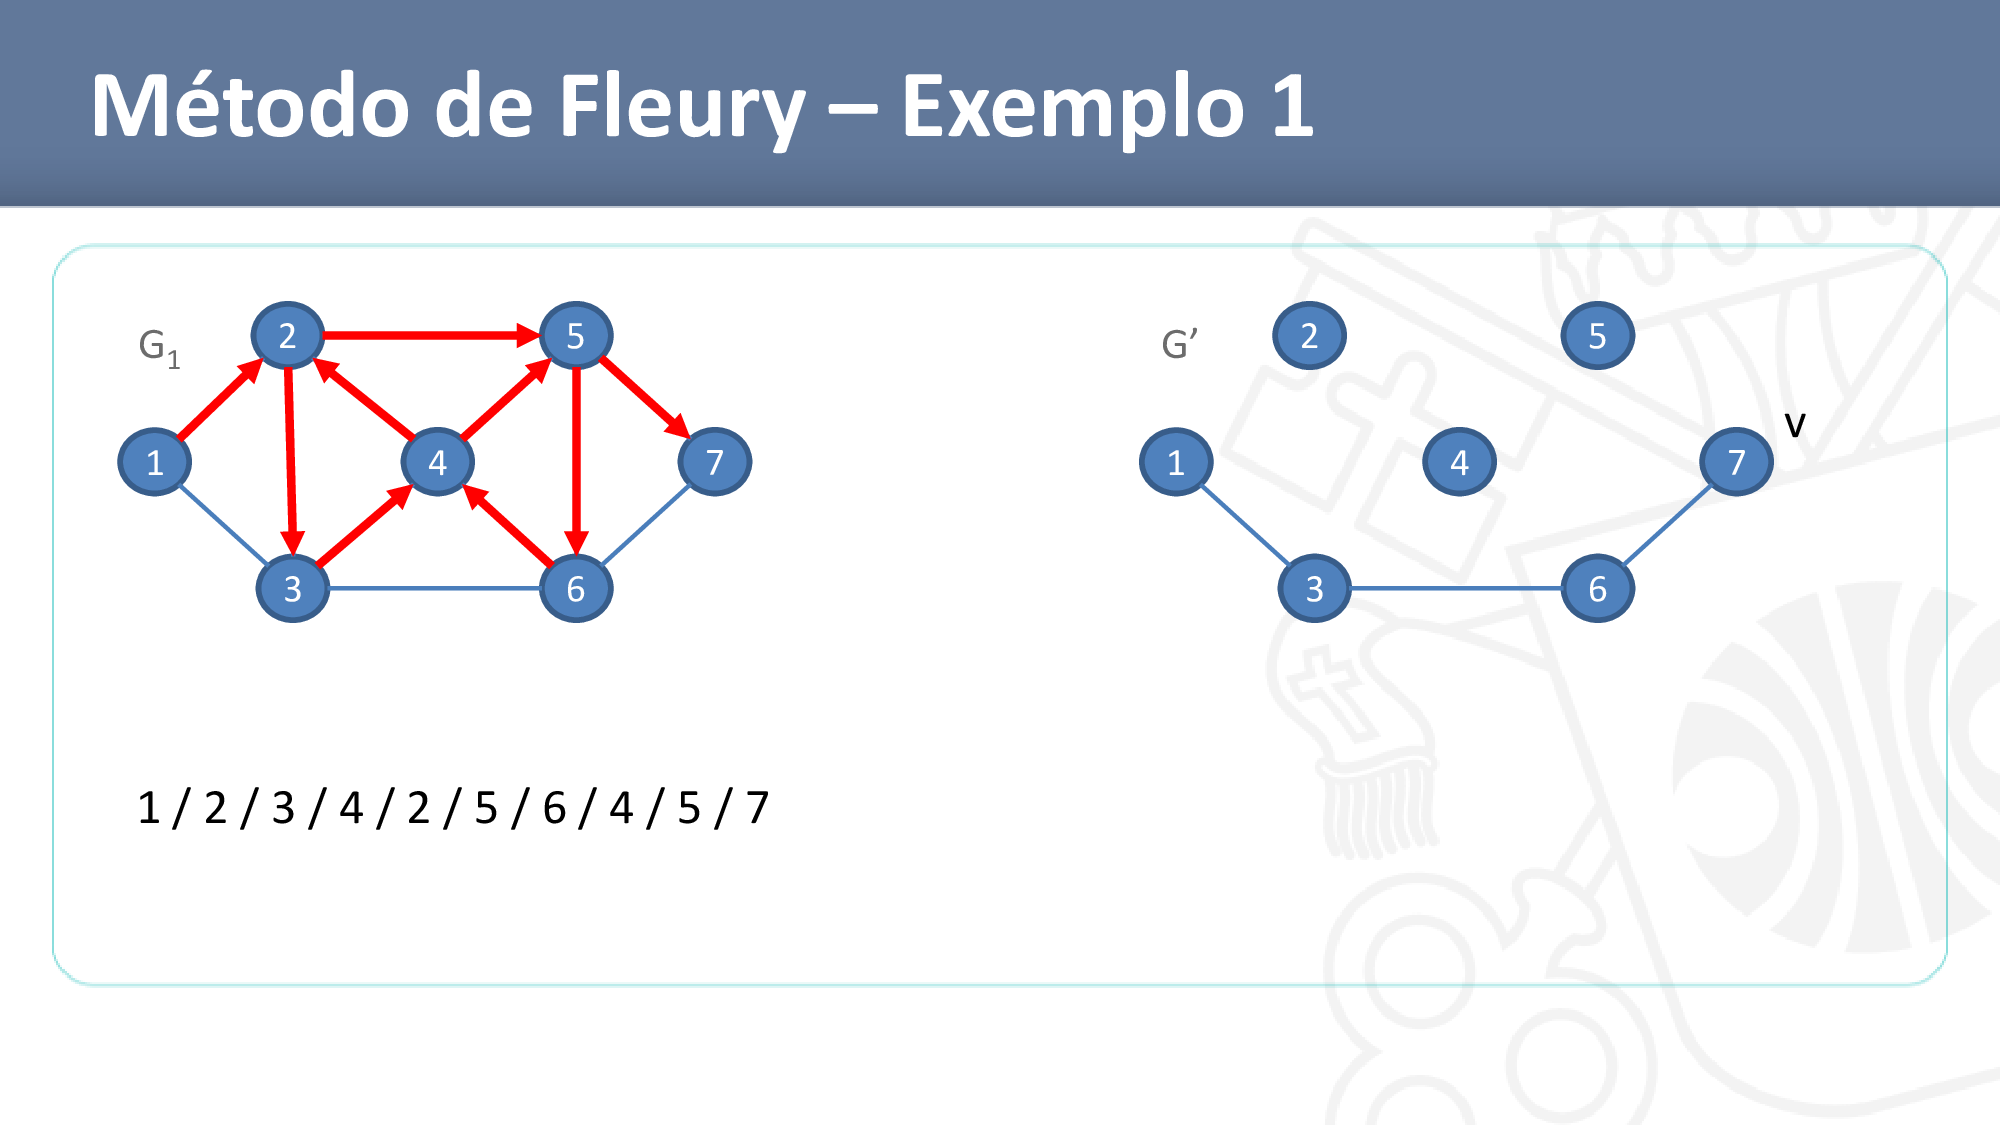
\includegraphics[width=\textwidth]{imagem/graficos/1a1455b7b9174768d1c6a0d41673e79dHTztESkzBtQzsXWu-43.png}
	\end{subfigure}
	\begin{subfigure}{.6\textwidth}
		\centering
		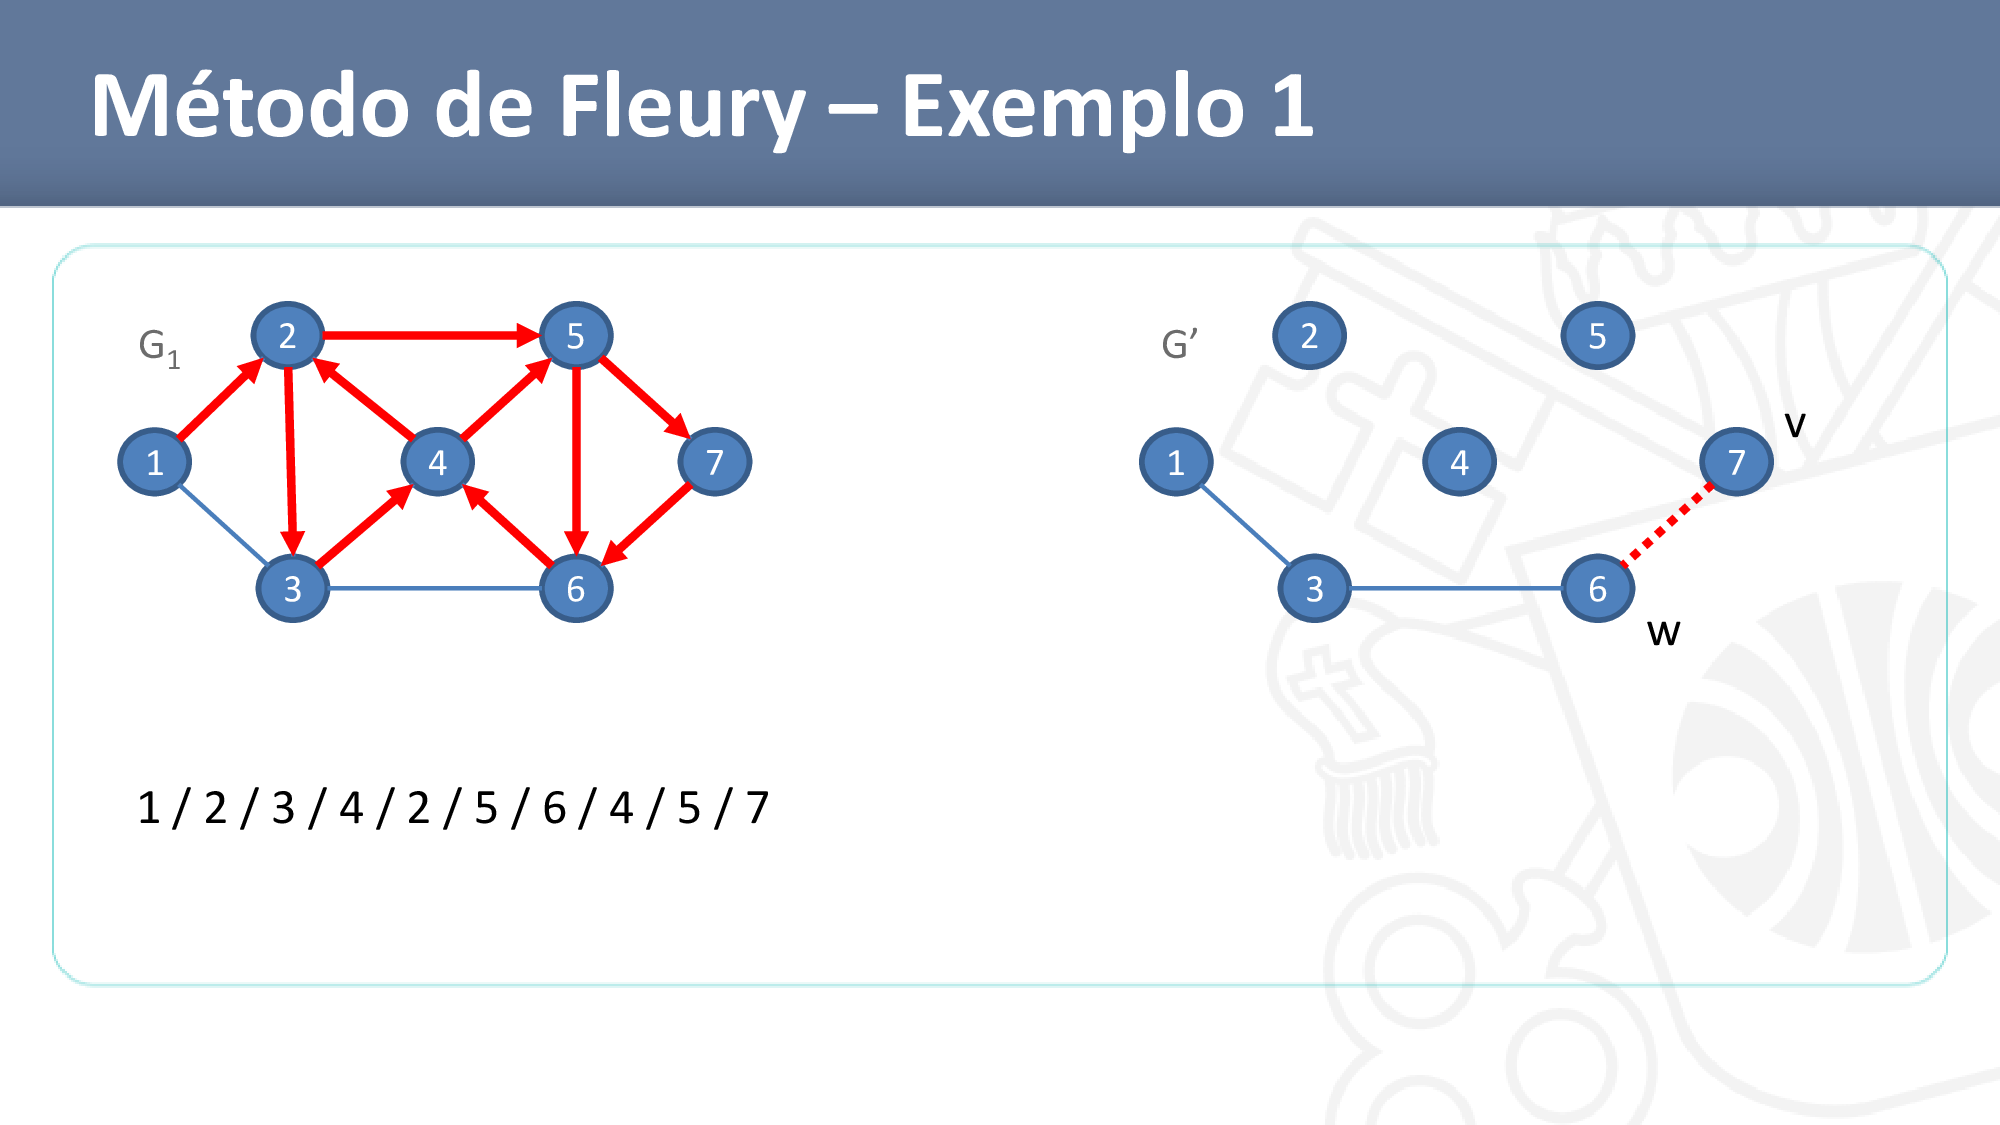
\includegraphics[width=\textwidth]{imagem/graficos/1a1455b7b9174768d1c6a0d41673e79dHTztESkzBtQzsXWu-44.png}
	\end{subfigure}
\end{figure}
\begin{figure}[H]
	\begin{subfigure}{.6\textwidth}
		\centering
		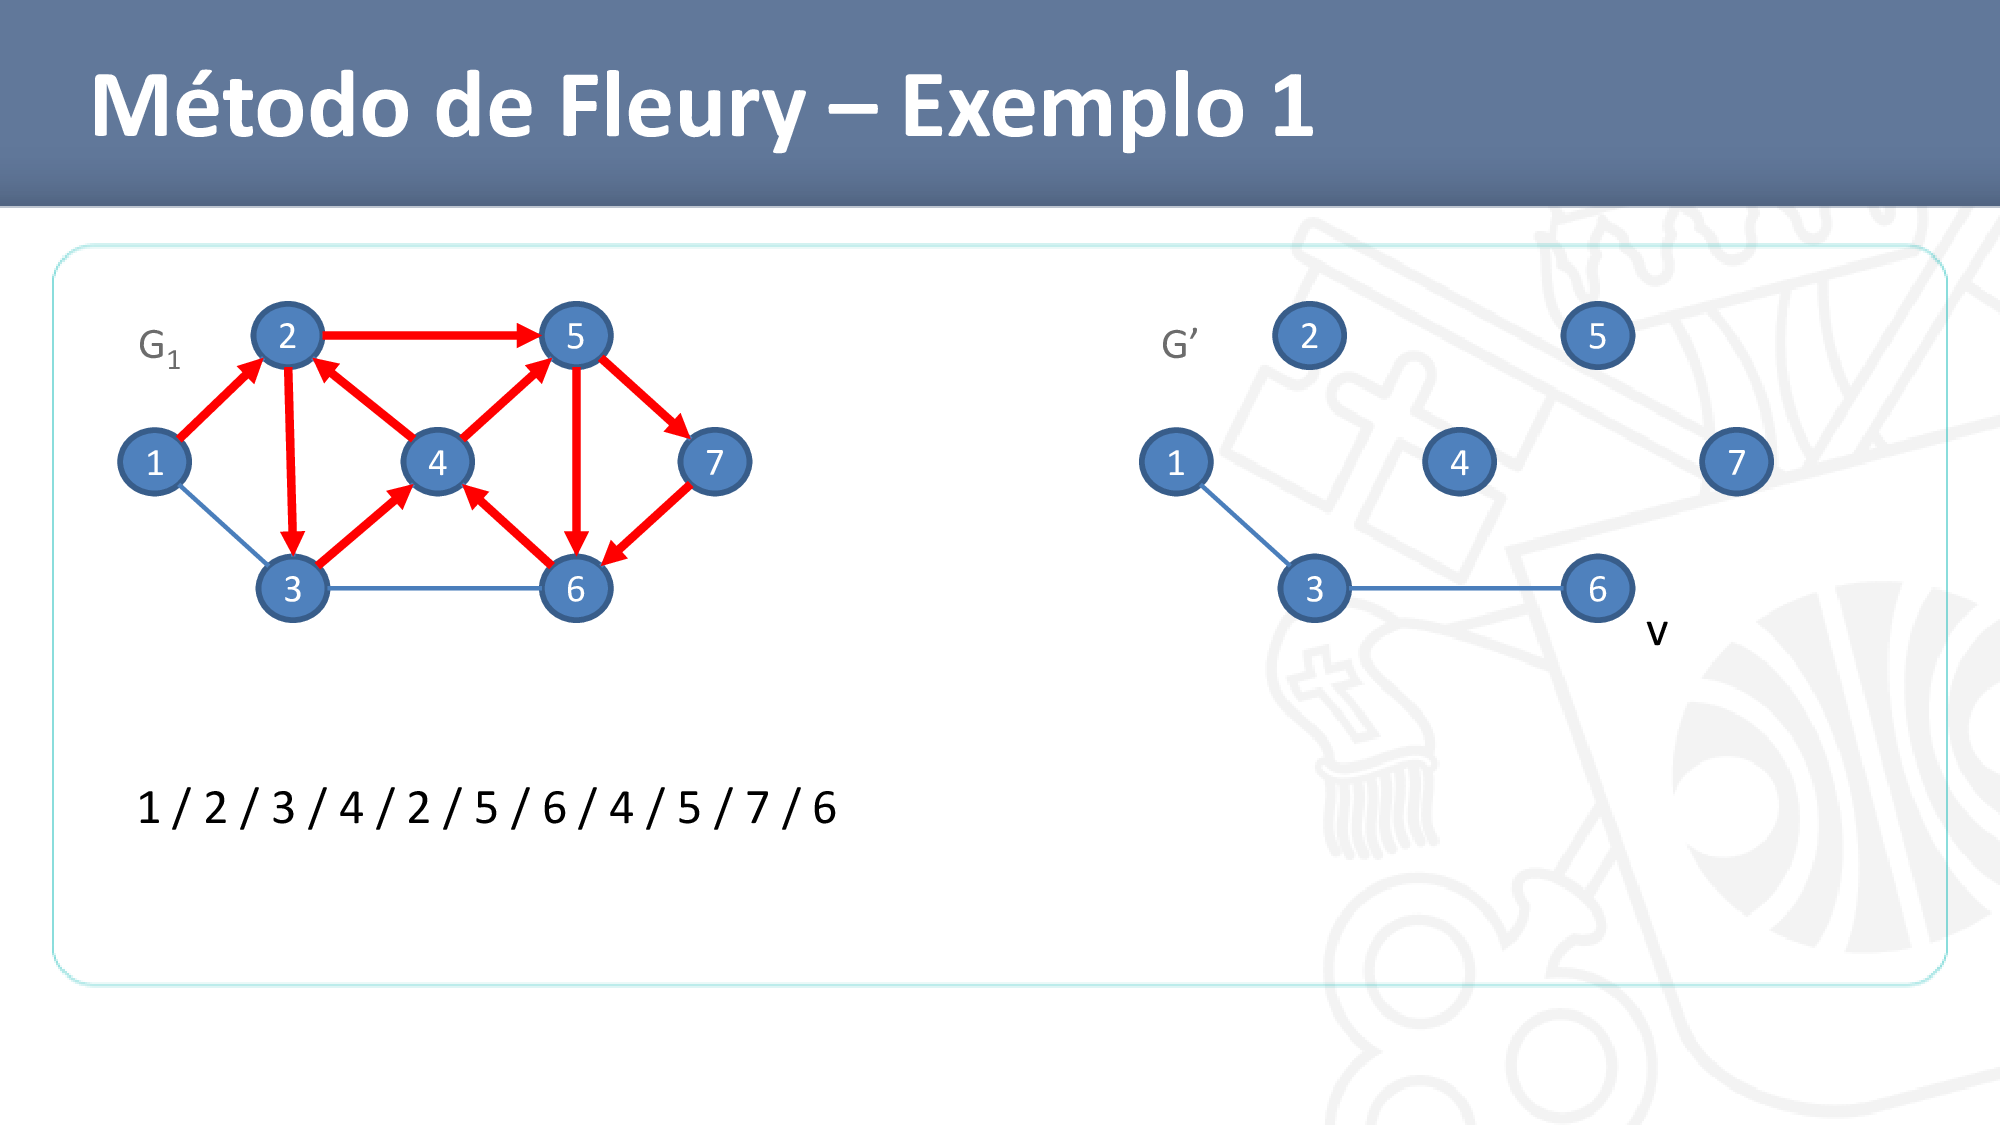
\includegraphics[width=\textwidth]{imagem/graficos/1a1455b7b9174768d1c6a0d41673e79dHTztESkzBtQzsXWu-45.png}
	\end{subfigure}
	\begin{subfigure}{.6\textwidth}
		\centering
		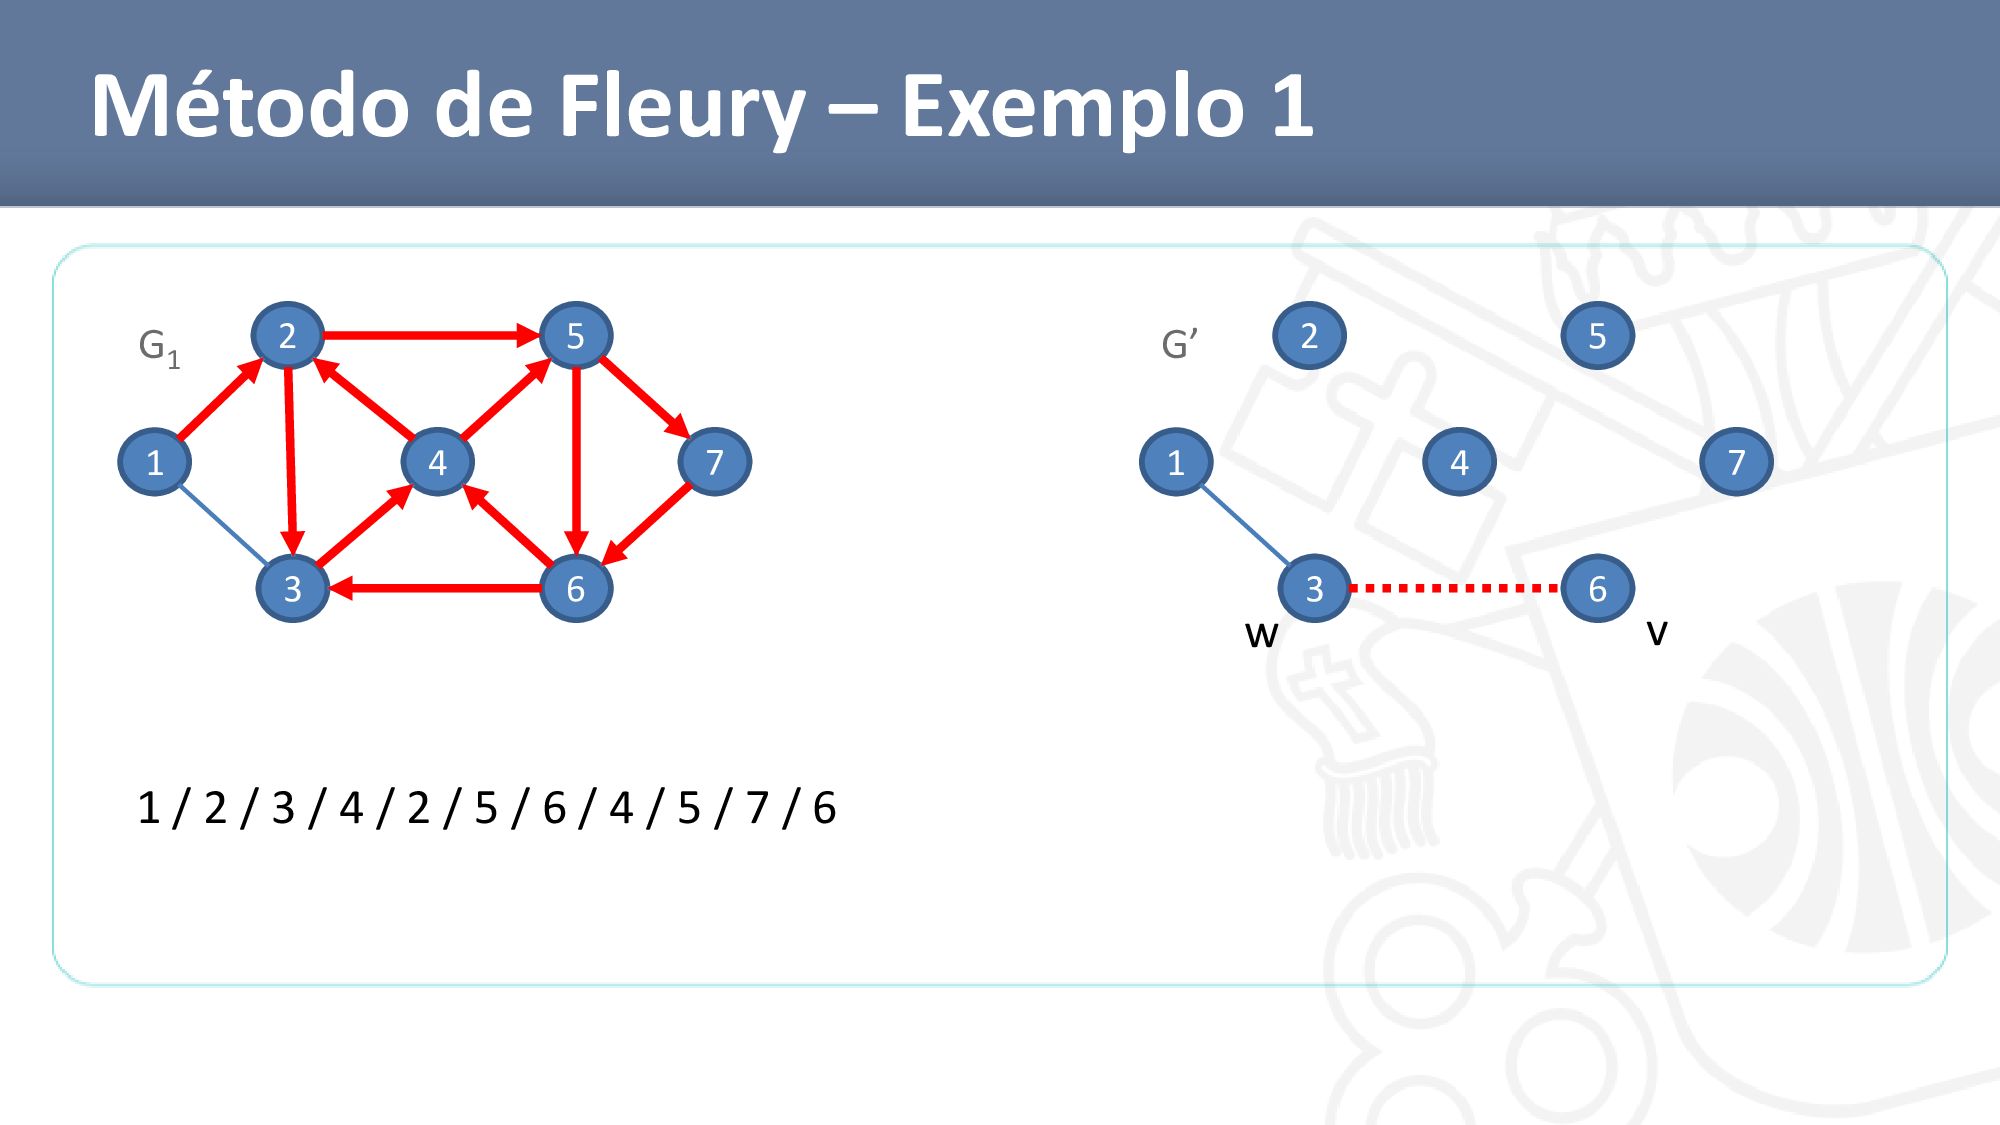
\includegraphics[width=\textwidth]{imagem/graficos/1a1455b7b9174768d1c6a0d41673e79dHTztESkzBtQzsXWu-46.png}
	\end{subfigure}
\end{figure}
\begin{figure}[H]
	\begin{subfigure}{.6\textwidth}
		\centering
		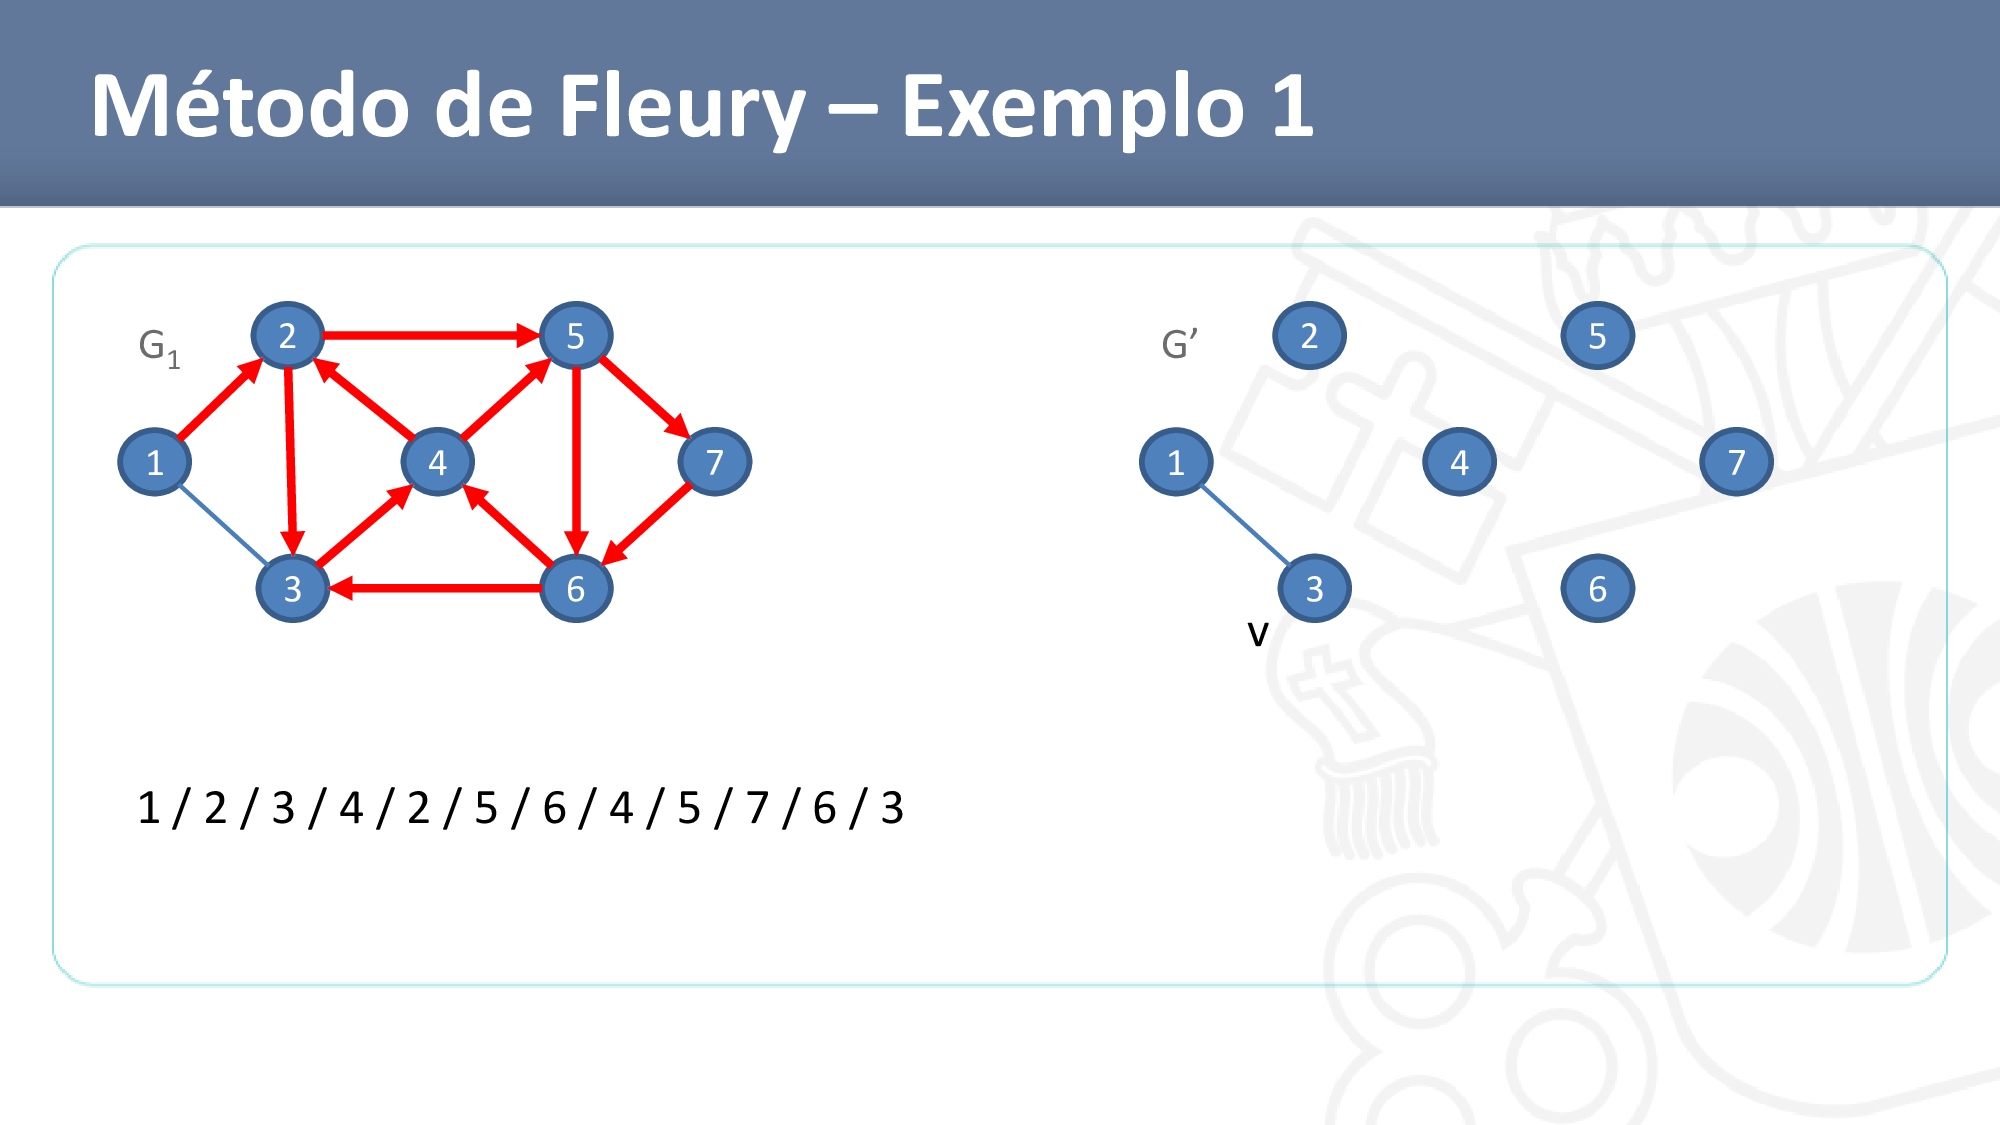
\includegraphics[width=\textwidth]{imagem/graficos/1a1455b7b9174768d1c6a0d41673e79dHTztESkzBtQzsXWu-47.png}
	\end{subfigure}
	\begin{subfigure}{.6\textwidth}
		\centering
		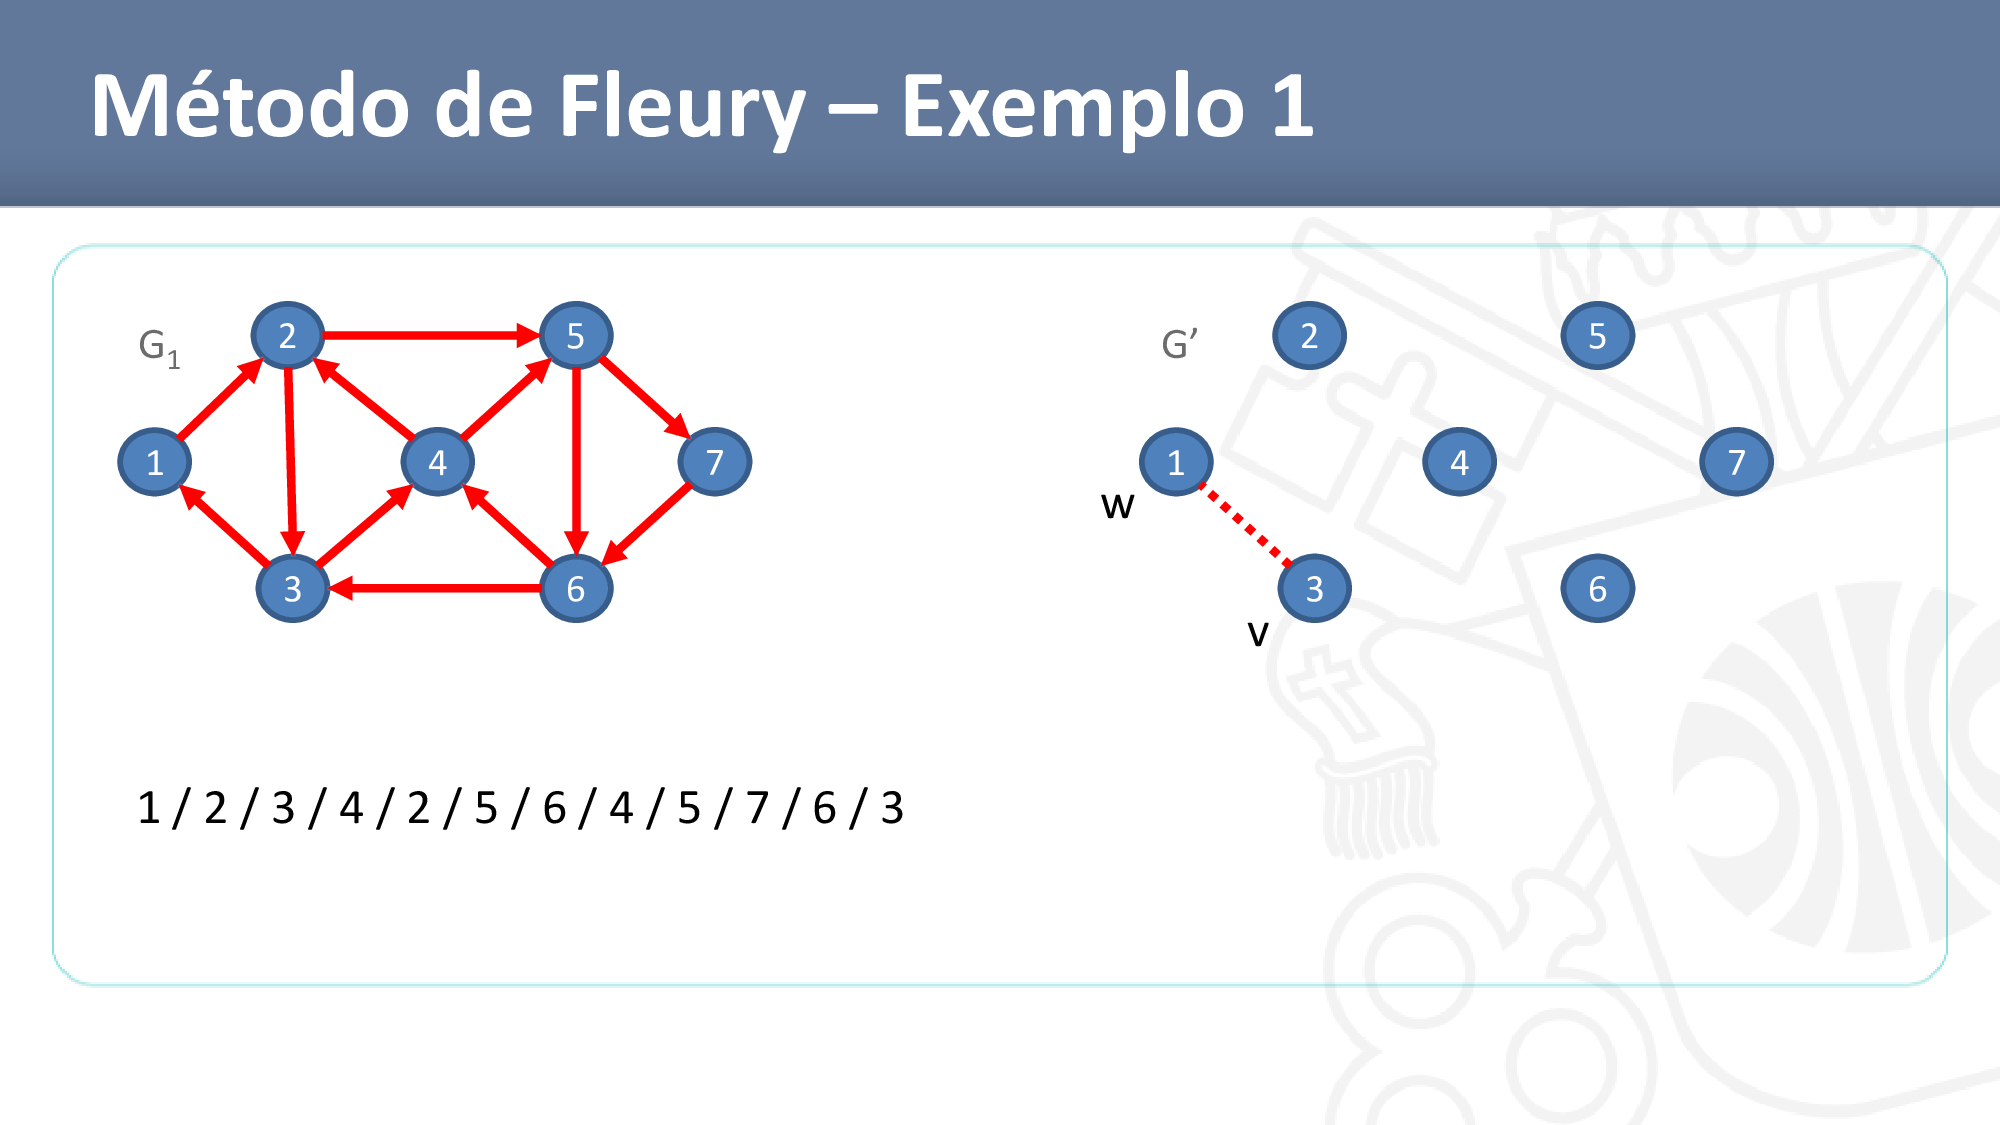
\includegraphics[width=\textwidth]{imagem/graficos/1a1455b7b9174768d1c6a0d41673e79dHTztESkzBtQzsXWu-48.png}
	\end{subfigure}
\end{figure}
\begin{figure}[H]
	\begin{subfigure}{.6\textwidth}
		\centering
		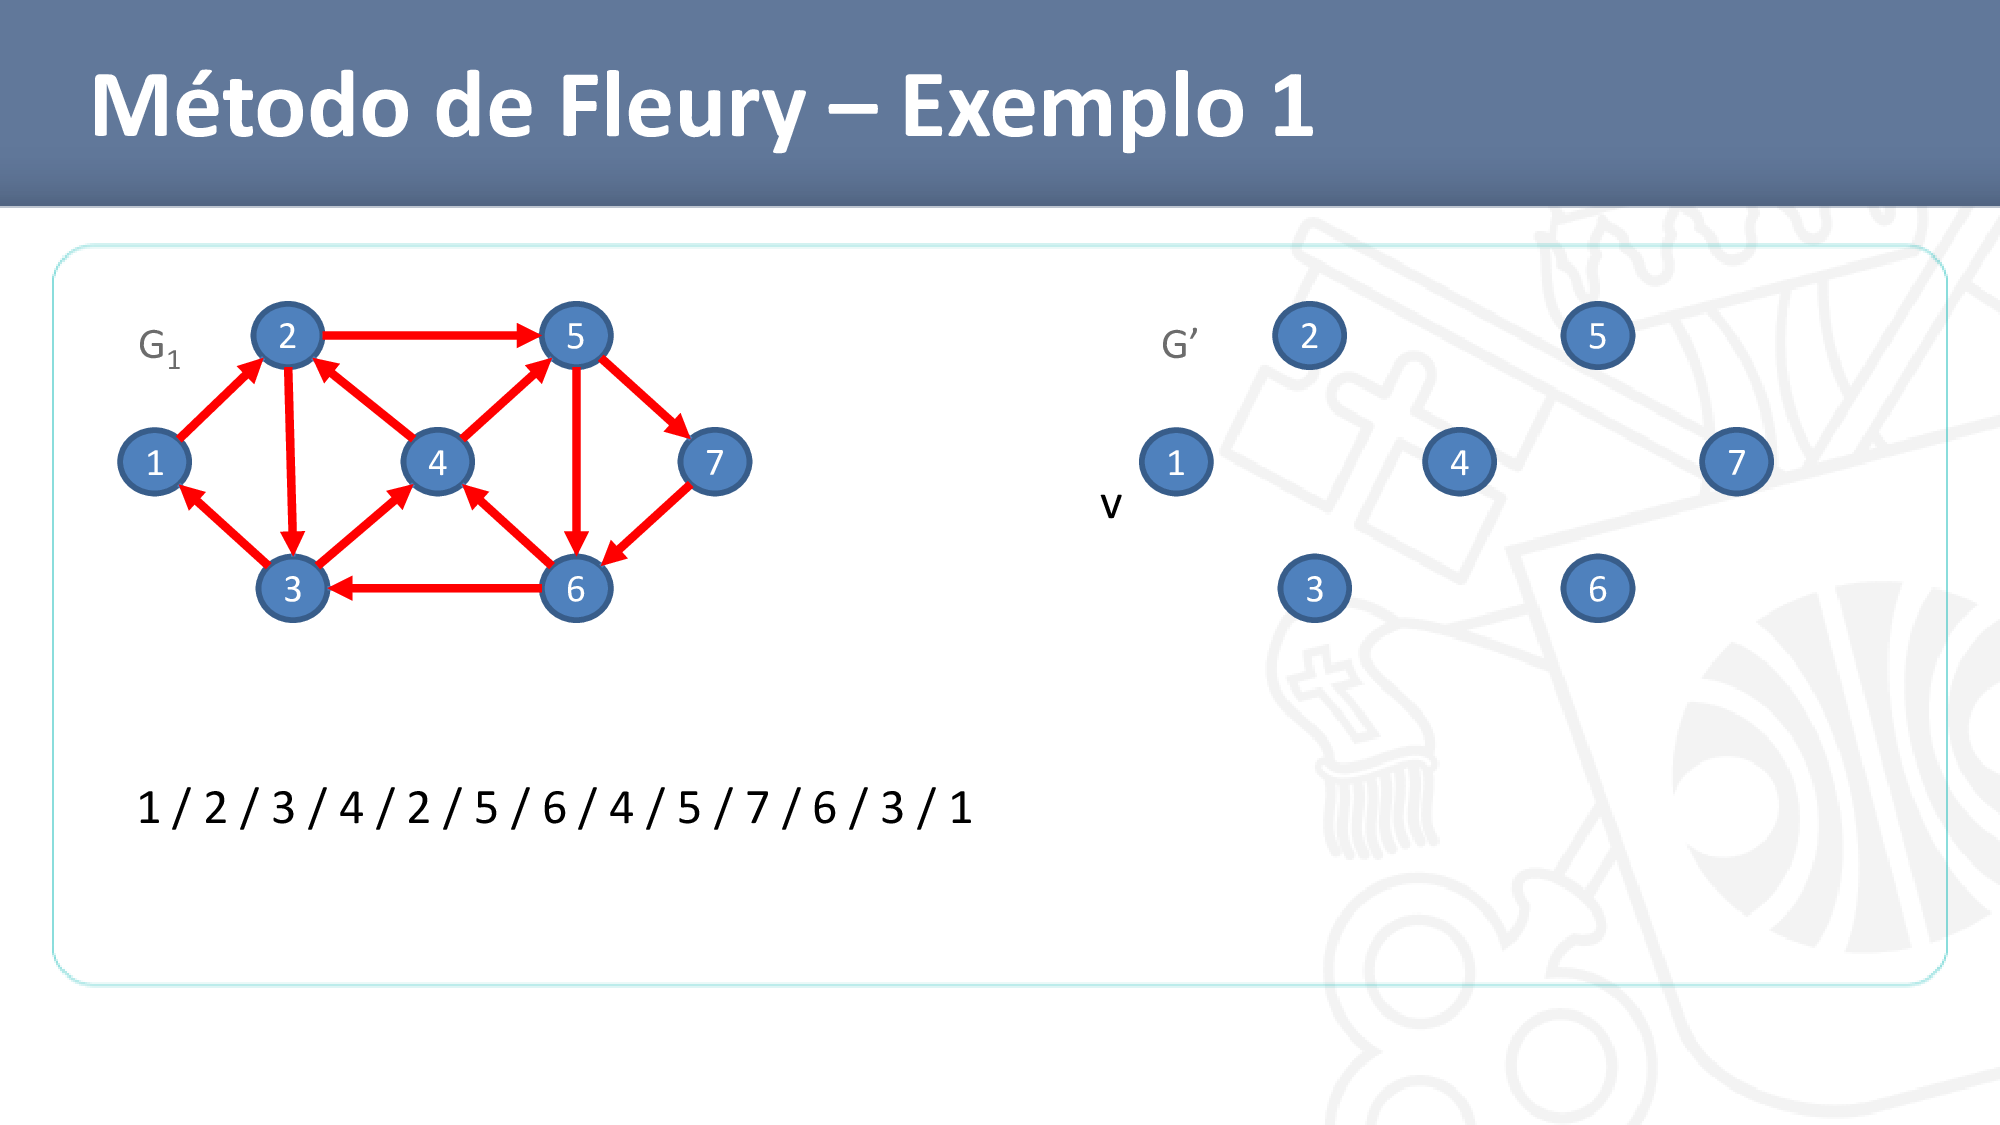
\includegraphics[width=\textwidth]{imagem/graficos/1a1455b7b9174768d1c6a0d41673e79dHTztESkzBtQzsXWu-49.png}
	\end{subfigure}
	\begin{subfigure}{.6\textwidth}
		\centering
		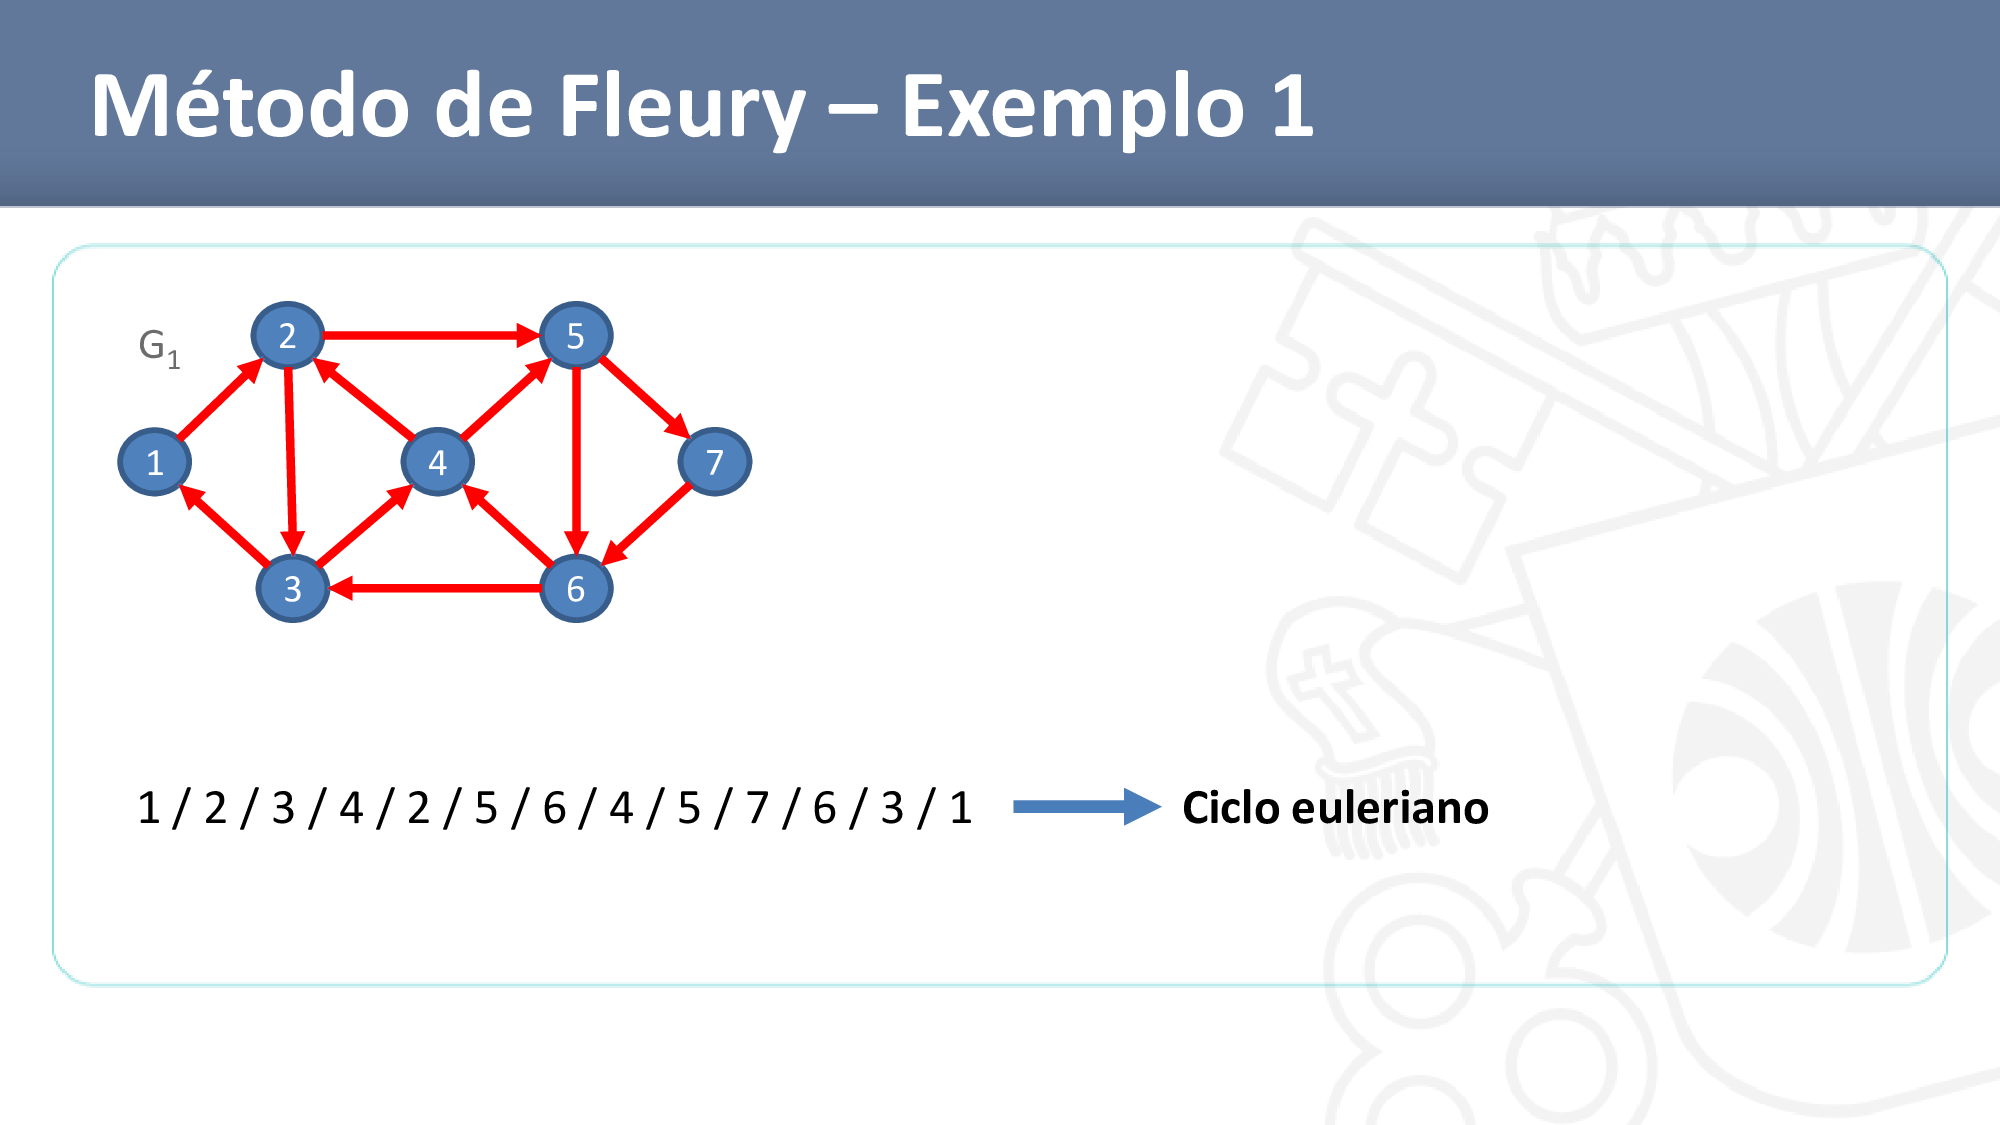
\includegraphics[width=\textwidth]{imagem/graficos/1a1455b7b9174768d1c6a0d41673e79dHTztESkzBtQzsXWu-50.png}
	\end{subfigure}
\end{figure}
